%%% Hlavní soubor. Zde se definují základní parametry a odkazuje se na ostatní části. %%%

%% Verze pro jednostranný tisk:
% Okraje: levý 40mm, pravý 25mm, horní a dolní 25mm
% (ale pozor, LaTeX si sám přidává 1in)
\documentclass[12pt,a4paper]{report}

\setlength{\hoffset}{-1in} %left margin will be 0, as hoffset is by default 1inch
\setlength{\voffset}{-1in} %analogous voffset
\setlength{\oddsidemargin}{4cm}
\setlength{\evensidemargin}{4cm}
\setlength{\topmargin}{25mm}
\setlength{\footskip}{3cm}
\setlength{\headheight}{0cm}
\setlength{\headsep}{0cm}
\setlength{\marginparwidth}{0cm}
\setlength{\marginparpush}{0cm}
\setlength{\textheight}{20.7cm}
\setlength{\textwidth}{14.5cm}
\let\openright=\clearpage


%\linespread{1.3}
%\renewcommand\baselinestretch{1.3} % riadkovanie jeden a pol

%% Pokud tiskneme oboustranně:
% \documentclass[12pt,a4paper,twoside,openright]{report}
% \setlength\textwidth{145mm}
% \setlength\textheight{247mm}
% \setlength\oddsidemargin{15mm}
% \setlength\evensidemargin{0mm}
% \setlength\topmargin{0mm}
% \setlength\headsep{0mm}
% \setlength\headheight{0mm}
% \let\openright=\cleardoublepage

%% Pokud pouľíváte csLaTeX (doporučeno):
%\usepackage{czech}
%% Pokud nikoliv:
%\usepackage[czech]{babel}
%\usepackage[T1]{fontenc}

%% Pouľité kódování znaků: obvykle latin2, cp1250 nebo utf8:
\usepackage[utf8]{inputenc}
\usepackage[T1]{fontenc}

%% Ostatní balíčky
\usepackage{graphicx}
\usepackage{amsthm}
\usepackage{amssymb}
\usepackage{amsmath}
\usepackage{todonotes}
\usepackage{algorithmic}
\usepackage[chapter]{algorithm}
\usepackage{subfig}
\usepackage{url}
\usepackage{multirow}
\usepackage{setspace}

\onehalfspacing

\newcommand{\myscale}{0.5}

\renewcommand{\algorithmicrequire}{\textbf{Input:}}
\renewcommand{\algorithmicensure}{\textbf{Output:}}

\renewcommand{\algorithmicforall}{\textbf{for each}}

\renewcommand{\algorithmiccomment}[1]{// #1}


% pekne pokope definujeme potrebne udaje
\def\mftitle{Efficient Detection of XML Integrity Constraints}
\def\mfthesistype{MASTER THESIS}
\def\mfkatedra{Department of Software Engineering}
\def\mfpracoviste{}
\def\mfauthor{Michal Švirec}
\def\mfadvisor{RNDr. Irena Mlýnková, Ph.D.}
\def\mfplacedate{Praha, 2011}

%% Balíček hyperref, kterým jdou vyrábět klikací odkazy v PDF,
%% ale hlavně ho pouľíváme k uloľení metadat do PDF (včetně obsahu).
%% POZOR, nezapomeňte vyplnit jméno práce a autora.
\usepackage[ps2pdf,unicode]{hyperref}   % Musí být za vąemi ostatními balíčky
\hypersetup{pdftitle=\mftitle}
\hypersetup{pdfauthor=\mfauthor}

%%% Drobné úpravy stylu

% Tato makra přesvědčují mírně oąklivým trikem LaTeX, aby hlavičky kapitol
% sázel příčetněji a nevynechával nad nimi spoustu místa. Směle ignorujte.
%\makeatletter
%\def\@makechapterhead#1{
%  {\parindent \z@ \raggedright \normalfont
%   \Huge\bfseries \thechapter. #1
%   \par\nobreak
%   \vskip 20\p@
%}}
%\def\@makeschapterhead#1{
%  {\parindent \z@ \raggedright \normalfont
%   \Huge\bfseries #1
%   \par\nobreak
%   \vskip 20\p@
%}}
%\makeatother

% Toto makro definuje kapitolu, která není očíslovaná, ale je uvedena v obsahu.
\def\chapwithtoc#1{
\chapter*{#1}
\addcontentsline{toc}{chapter}{#1}
}

\begin{document}

% Trochu volnějąí nastavení dělení slov, neľ je default.
%\lefthyphenmin=2
%\righthyphenmin=2

%%% Titulní strana práce

\pagestyle{empty}
\begin{center}

\large

Charles University in Prague

\medskip

Faculty of Mathematics and Physics

\vfill

{\bf\Large \mfthesistype}

\vfill

\centerline{\mbox{
\includegraphics[width=60mm]{logo.eps}}}

\vfill
\vspace{5mm}

{\LARGE \mfauthor}

\vspace{15mm}

% Název práce přesně podle zadání
{\LARGE\bfseries \mftitle}

\vfill

% Název katedry nebo ústavu, kde byla práce oficiálně zadána
% (dle Organizační struktury MFF UK)
\mfkatedra

\vfill

\begin{tabular}{rl}

Supervisor of the master thesis: & \mfadvisor \\
\noalign{\vspace{2mm}}
Study programme: & Informatics \\
\noalign{\vspace{2mm}}
Specialization: & Software Systems \\
\end{tabular}

\vfill

% Zde doplňte rok
\mfplacedate

\end{center}

\newpage

%%% Následuje vevázaný list -- kopie podepsaného "Zadání diplomové práce".
%%% Toto zadání NENÍ součástí elektronické verze práce, nescanovat.

%%% Na tomto místě mohou být napsána případná poděkování (vedoucímu práce,
%%% konzultantovi, tomu, kdo zapůjčil software, literaturu apod.)

\openright

\noindent
I would like to thank my supervisor RNDr. Irena Mlýnková, Ph.D., for her helpful advices, corrections and suggestions.

\newpage

%%% Strana s čestným prohláąením k diplomové práci

\vglue 0pt plus 1fill

\noindent
I declare that I carried out this master thesis independently, and only with the cited
sources, literature and other professional sources.

\medskip\noindent
I understand that my work relates to the rights and obligations under the Act No.
121/2000 Coll., the Copyright Act, as amended, in particular the fact that the Charles
University in Prague has the right to conclude a license agreement on the use of this
work as a school work pursuant to Section 60 paragraph 1 of the Copyright Act.

\vspace{10mm}

\hbox{\hbox to 0.5\hsize{%
In ........ date ............
\hss}\hbox to 0.5\hsize{%
Signature
\hss}}

\vspace{20mm}
\newpage

%%% Povinná informační strana diplomové práce

\vbox to 0.5\vsize{
\setlength\parindent{0mm}
\setlength\parskip{5mm}

Název práce:
Efektívna detekcia integritných obmedzení v XML
% přesně dle zadání

Autor:
\mfauthor

Katedra:  % Případně Ústav:
Katedra softwarového inženýrství
% dle Organizační struktury MFF UK

Vedoucí diplomové práce:
\mfadvisor

% dle Organizační struktury MFF UK, případně plný název pracoviątě mimo MFF UK

Abstrakt:
Znalosť integritných obmedzení v XML dátach je jeden z dôležitých aspektov ich spracovania. Avšak aj keď tieto integritné obmedzenia pre dané dáta poznáme, je častým javom, že dané dáta sú voči ním nekonzistentné. Z tohto dôvodu vznikla snaha detekovať tieto nekonzistentosti dát a následne ich opravovať. Táto práca rozširuje a zdokonaľuje doterajšie prístupy opráv XML dokumentov porušujúcich definované integritné obmedzenia, konkrétne takzvané funkčné závislosti. Práca prináša algoritmus začleňujúci váhový model a taktiež zapája užívateľa do procesu hľadania a následného aplikovania vhodnej opravy nekonzistentných XML dokumentov. Súčasťou práce sú experimentálne výsledky.

% abstrakt v rozsahu 80-200 slov; nejedná se vąak o opis zadání diplomové práce

Klíčová slova: XML, funkčná závislosť, porušenie funkčných závislostí, oprava porušení
% 3 aľ 5 klíčových slov


\vss}


\newpage

\vbox to 0.5\vsize{
\setlength\parindent{0mm}
\setlength\parskip{5mm}

Title:
\mftitle
% přesný překlad názvu práce v angličtině

Author:
\mfauthor

Department:
\mfkatedra
% dle Organizační struktury MFF UK v angličtině

Supervisor:
\mfadvisor
% dle Organizační struktury MFF UK, případně plný název pracoviątě
% mimo MFF UK v angličtině

Abstract:
Knowledge of integrity constraints covered in the XML data is an important aspect of efficient data processing. However, although the integrity constraints are defined for the given data, it is a common phenomenon that data violate the predefined set of constraints. Therefore detection of these inconsistencies and consecutive repair has emerged. This work extends and refines recent approaches to repairing XML documents violating defined set of integrity constraints, specifically so-called functional dependencies. The work propose the repair algorithm incorporating the weight model and also involve user into the process of detection and subsequent application of appropriate repair of inconsistent XML documents. Experimental results are part of the work.
% abstrakt v rozsahu 80-200 slov v angličtině; nejedná se vąak o překlad
% zadání diplomové práce

Keywords: XML, functional dependency, functional dependencies violations, violations repair
% 3 aľ 5 klíčových slov v angličtině

\vss}

\newpage

%%% Strana s automaticky generovaným obsahem diplomové práce. U matematických
%%% prací je přípustné, aby seznam tabulek a zkratek, existují-li, byl umístěn
%%% na začátku práce, místo na jejím konci.

\openright
\pagestyle{plain}

\renewcommand\thepage{}
\tableofcontents
\newpage
\renewcommand\thepage{\arabic{page}}

\setcounter{page}{1}



\newtheorem{theorem}{Theorem}
\theoremstyle{definition}
\newtheorem{define}{Definition}[chapter]	% Definice nečíslujeme, proto "*"
\newtheorem{example}{Example}


%%% Jednotlivé kapitoly práce jsou pro přehlednost uloľeny v samostatných souborech
\include{uvod}
\chapter{Introduction}

Nowadays, one of the most largely used standards for information representation and data exchange on the Internet is the eXtensible Markup Language (XML) \cite{xml}. While XML as a markup language provides syntactic flexibility, the structure of an XML document is described with a so-called XML schema language. The two most popular XML schema languages proposed by W3C\footnote{The World Wide Web Consorcium, \url{http://www.w3.org}} are Document Type Definition (DTD) \cite{xml} and XML Schema Definition (XSD) \cite{xsd1,xsd2,xsd3}. They support some kind of semantic content (e.g., keys and foreign keys), but for improvement of semantic expressiveness integrity constraints for XML \cite{ic} have been defined.

However, similarly to the problem of schemas, also the problem of detection of integrity constrains has two distinct aspects. First, if integrity constraints are not explicitly expressed, they need to be detected from the given set of data. Second, if integrity constraints are expressed, XML document may not be consistent with respect to them and this needs to be detected (checking the satisfaction of integrity constraint in an XML document). Moreover, the detected XML data inconsistency needs to be repaired. In this thesis we choose the latter aspect of detection of integrity constraints along with the repair of the inconsistent XML document. Since several different classes of integrity constraints have been defined for XML, we choose so-called functional dependency (FD) \cite{fd} which is the most common semantic constraint used in relational databases.

The problem of checking the satisfaction of functional dependencies in an XML document is studied in \cite{satifFD}. Also algorithms computing a repair applied to an XML document such that functional dependencies will be satisfied again have been proposed \cite{RepAndConsistentAnswer, QueryXML, ImprovingXML}.

\section{Aim of the Thesis}

The aim of this thesis is to propose an algorithm repairing XML functional dependency violations for a given XML document and a set of functional dependencies. It analyses recent approaches and discusses their advantages and disadvantages. The focus of the thesis is to incorporate a weight model, to involve the user the process of finding and applying the repair and to find out how this interaction helps. An important part of the thesis is an experimental implementation of the proposed algorithm and its experimental evaluation.

\section{Structure of the Thesis}

Chapter 2 introduces basic definitions which are necessary for further chapters. Chapter 3 presents recent approaches of repairing XML functional dependency violations. In Chapter 4 the main algorithm is proposed. Chapter 5 contains details of the experimental implementation. Experimental result are presented in Chapter 6. Finally, Chapter 7 contains a conclusion and several suggestions for future work.

\chapter{Basic Definitions}

In this chapter basic definitions necessary in the following chapters are placed. The definitions are taken from \cite{RepAndConsistentAnswer, QueryXML, ImprovingXML}.


\section{XML Trees and DTDs}
\begin{define}[Tree]
Being given an alphabet of nodes $\mathbb{N}$ and an alphabet of node labels $\Sigma$, a {\sl tree} $T$ over $\mathbb{N}$ and $\Sigma$ is a tuple $(r_T, N_T, E_T, \lambda_T)$, where $N_T \subseteq \mathbb{N}$ is the set of nodes, $\lambda_T : N_T \to \Sigma$ is a node labelling function, $r_T \in N_T$ is the distinguished root of $T$, and $E_T \subseteq N_T \times N_T$ is a set of edges such that starting from any node $n_i \in N_T$ it is possible to reach any other node $n_j \in N_T$, walking through a sequence of edges $e_1,\dots,e_k$ which are connected and acyclic.\qed
\end{define}

\noindent Let us also denote the set of leaf nodes as $Leaves(T)$ and the set of trees defined over an alphabet of node labels $\Sigma$ as $T_\Sigma$.

\begin{define}[XML Tree]\label{xmlTree}
{\sl XML tree} is a pair $XT=\langle T,\delta \rangle$, where:
\renewcommand{\labelenumi}{\roman{enumi})}
	\begin{enumerate}
		\item $T = (r, N, E, \lambda)$ is a tree from $T_{\tau\cup\alpha\cup\{S\}}$, where $\tau$ is a tag alphabet, $\alpha$ is an attribute name alphabet and $S$ is a symbol not belonging to $\tau\cup\alpha$ (representing \texttt{\#PCDATA} content of elements)$;$
		\item given a node $n$ of $T$, $\lambda(n) \in \alpha \cup \{S\} \Leftrightarrow n \in Leaves(T);$
		\item $\delta : Leaves(T) \rightarrow Str$ where $Str$ is a string alphabet is a function associating a (string) value to every leaf of $T$.
	\end{enumerate}\qed
\end{define}

\begin{example}\label{example1ref}
Consider the following XML document representing a collection of books. Its graphical representation as an XML tree is in Fig. \ref{example1}.
\begin{verbatim}
<bib>
  <book>
    <written_by>
      <author ano="A1">
        <name>John Writer</name>
      </author>
      <author ano="A1">
        <name>Eric Seller</name>
      </author>
    </written_by>
    <title>Some title</title>
  </book>
  <book>
    <written_by>
      <author ano="A2">
        <name>Adam Publisher</name>
      </author>
    </written_by>
    <title>Some title 2</title>
  </book>
</bib>
\end{verbatim}

The nodes of an XML tree have a label denoting the tag name of the element and unique element identifier in brackets. Leaf nodes are either an attribute or the textual content of an element. The label of a textual node contains string contained inside of element and unique element identifier. The label of an attribute node contains in addition to textual node the name of the attribute.\qed
\end{example}

\begin{figure}[h]
    \centering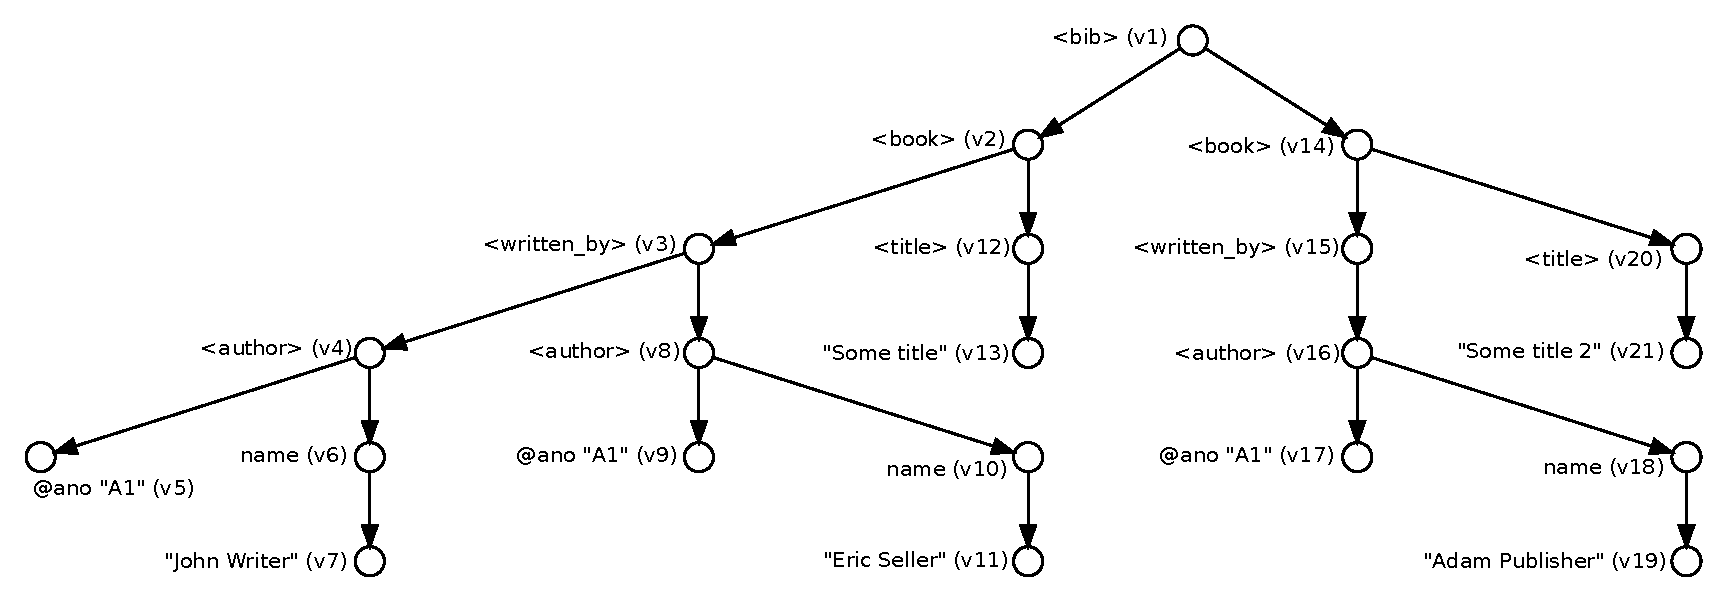
\includegraphics[width=\textwidth]{example1-new}
	\caption{An XML Tree} \label{example1}
\end{figure}

\begin{define}[DTD]\label{dtdDef}
{\sl DTD} is a tuple $D = (\tau, \alpha, P, R, rt)$ where:
\renewcommand{\labelenumi}{\roman{enumi})}
\begin{enumerate}
	\item $\tau$ and $\alpha$ are of the same definition as in the \emph{XML tree}
    \item $P$ is the set of \emph{element type definitions}
    \item $R$ is the set of \emph{attribute lists}
    \item $rt \in \tau$ is the tag of the document root element.
\end{enumerate}
\qed
\end{define}

\begin{define}[Path Expression]
A {\sl path expression} is an expression of the form $p = ('/' | '//')s_1 \dots ('/'|'//')s_m$ where $s_1, \dots, s_{m-1} \in \tau$, and $s_m \in \tau \cup \alpha \cup \{S\}$.\qed
\end{define}

\begin{define}[Path]
{\sl Path} p on a DTD $D = (\tau, \alpha, P, R, rt)$ is a sequence $p = s_1, \dots, s_m$ of symbols in $\tau \cup \alpha \cup \{S\}$ such that:
\renewcommand{\labelenumi}{\roman{enumi})}
	\begin{enumerate}
		\item $s_1=rt$;
		\item for each $i$ in $2..m-1$, $s_i \in \tau$ and $s_i$ appears in the element type definition of $s_{i-1}$;
		\item $s_m \in \alpha \Rightarrow s_m$ appears in the attribute list of $s_{m-1}$;
		\item $s_m \in \tau \cup \{S\} \Rightarrow s_m$ appears in the element type definition of $s_{m-1}$.
	\end{enumerate}\qed
\end{define}

As we have defined a \emph{path} on a DTD $D$, let us denote $paths(D)$ as the set of all paths which can be defined on a DTD $D$. Also, another important notion is $p(XT)$ (or $\{[\![p]\!]\}$), which is the set of nodes from XML tree $XT$ conforming to DTD $D$, which can be reached by the path $p \in paths(D)$, starting from the root of $XT$. The set of nodes reachable from a node $v$ following path $p$ is denoted as $\{v[\![p]\!]\}$. When there is only one node in $\{v[\![p]\!]\}$, we use $v[\![p]\!]$ to denote this node. Moreover, let $XT.p$ denote the \emph{answer} of the path $p$ applied on $XT$ that is:
\begin{itemize}
	\item if $p \in EPath(D)$, where $EPath(D)$ denotes the set of the paths whose last symbol denotes an element, then $XT.p = p(XT)$
	\item if $p \in StrPath(D)$, where $StrPath(D)$ denotes the set of paths whose last symbol denotes either the textual content of an element or an
attribute, then $XT.p = \{\delta_T(x)|x \in p(XT)\}$.
\end{itemize}

\begin{example}\label{pathExample}
Consider the XML tree $XT$ from Example \ref{example1ref} conforming the DTD $D$ defined below, which is representing a collection of books.
\begin{verbatim}
<!ELEMENT bib (book+)>
<!ELEMENT book (written_by, title)>
<!ELEMENT written_by (author+)>
<!ELEMENT author (name)>
<!ATTLIST author ano CDATA>
<!ELEMENT name PCDATA>
<!ELEMENT title PCDATA>
\end{verbatim}

The set $paths(D)$ contains the following paths:
\begin{align}
paths(D) &= \left\{/bib, /bib/book, /bib/book/written\_by,\right.\nonumber\\
&\qquad \left. /bib/book/written\_by/author, \right.\nonumber\\
&\qquad \left. /bib/book/written\_by/author/name, \right.\nonumber\\
&\qquad \left. /bib/book/written\_by/author/name/S, \right.\nonumber\\
&\qquad \left. /bib/book/written\_by/author/@ano, \right.\nonumber\\
&\qquad \left. /bib/book/title, /bib/book/title/S\nonumber\right\}
\end{align}\qed
\end{example}

\section{Integrity Constraints}

Before defining of the XML integrity constraint, let us introduce some notation used in the definition. A \emph{path atom} is an expression of the form $[x_1]p[x_2]$, where $p$ is a path expression, $x_1$ and $x_2$ are terms, and $x_1 \not \in Str$.\\
A conjunction of path and built-in atoms $C = [X_1]p_1[Y_1] \cap \dots \cap [X_n]p_n[Y_n] \cap U_1\theta_1 V_1 \cap \dots \cap U_k \theta_k V_k$ is said to be \emph{safe} if all variables in $C$ are \emph{range restricted}, i.e. if
\begin{itemize}
 	\item for every $[X_i]p_i[Y_i]$, either $X_i$ is a constant (node identifier of a string), or there is some $[X_j]p_j[Y_j]$ in $C$ where $X_j$ is range restricted;
    \item for every built-in term $U_i\theta_i V_i$ occurring in $C$, if $\theta_i$ is equal to $"="$ then at least one of the two terms is range restricted; otherwise both $U_i$ and $V_i$ must be range restricted.
 \end{itemize}

A rootless tree formula is an expression of the form $p(\Phi_1 \land \dots \land \Phi_k)$ where $\Phi_i$ is a rootless path formula (expression of the form $p[y]$ where $p$ is a path expression and $y$ is a term) or a rootless tree formula and $p$ is a path expression. A tree atom is an expression of the form $[x]T$ where $T$ is a rootless tree formula and $x$ is a term.

\begin{define}[XML Integrity Constraint]\label{integConstr}
An {\sl XML constraint} is a formula of the form: $$(\forall X)[\Phi(X)\supset (\exists Y_1)\Psi_1(X,Y_1) \lor \dots \lor (\exists Y_k)(X,Y_k)]$$
where $X,Y_1,\dots, Y_k$ denote distinct sets of universally and existentially quantified variables, $\Phi(X)$ and $\Phi(X) \land \Psi_i(X, Y_i) (\forall i \in [1..k])$ are safe conjunctions of built-in and tree atoms.\qed
\end{define}

\begin{example}
Consider the XML tree $XT$ from Example \ref{example1ref}. Thereafter the integrity constraint that there must exist at least two books differents titles is expressed as

\begin{align*}
\forall(X)&[[root]/bib[X] \supset\\
&\exists(Z_1, Z_2)([X]/book/title/S[Z_1] \land [X]/book/title/S[Z_2] \land Z_1 \not = Z_2)]
\end{align*}
\end{example}

\section{Functional Dependencies}

Since different approaches uses slightly different representation of an XML document, also the definition of functional dependencies differs, too. This is the reason why we introduce two different definitions in this section.

\subsection{Functional Dependency 1}

In a relational database, a correspondence between values $A$ and $B$ in the tuple of $D$ models the functional dependency denoted as $A \rightarrow B$. Since in XML there is no such standard tuple concept, the concept of XML tree tuples is introduced, corresponding to the concept of tuples in relational databases.

\begin{define}[Tree Tuple]\label{treeTuple}
Being given an XML tree $XT$ conforming to DTD $D$, a {\sl tree tuple} $t$ of $XT$ is a maximal sub-tree of $XT$ such that for every path $p \in paths(D)$, $t.p$ contains at most one element.\qed
\end{define}

\begin{example}
Consider the XML tree $XT$ in Fig. \ref{example1}. The subtrees of $XT$ shown in Fig. \ref{tuples} are tree tuples, and the subrees in Fig. \ref{nottuples} are not.

\begin{figure}[H]
    \centering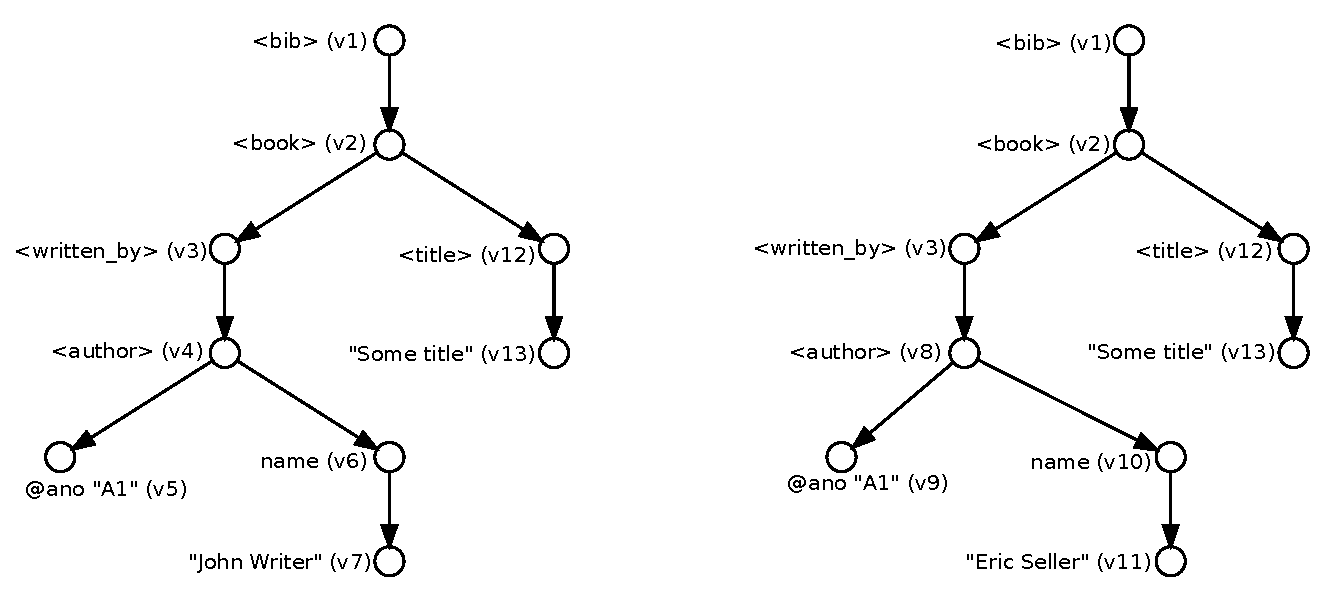
\includegraphics[width=\textwidth]{tuples}
	\caption[Two tree tuples of the XML tree]{Two tree tuples of the XML tree in Fig. \ref{example1}} \label{tuples}
\end{figure}

\begin{figure}[H]
    \centering
    \subfloat[]{\label{nottuple1}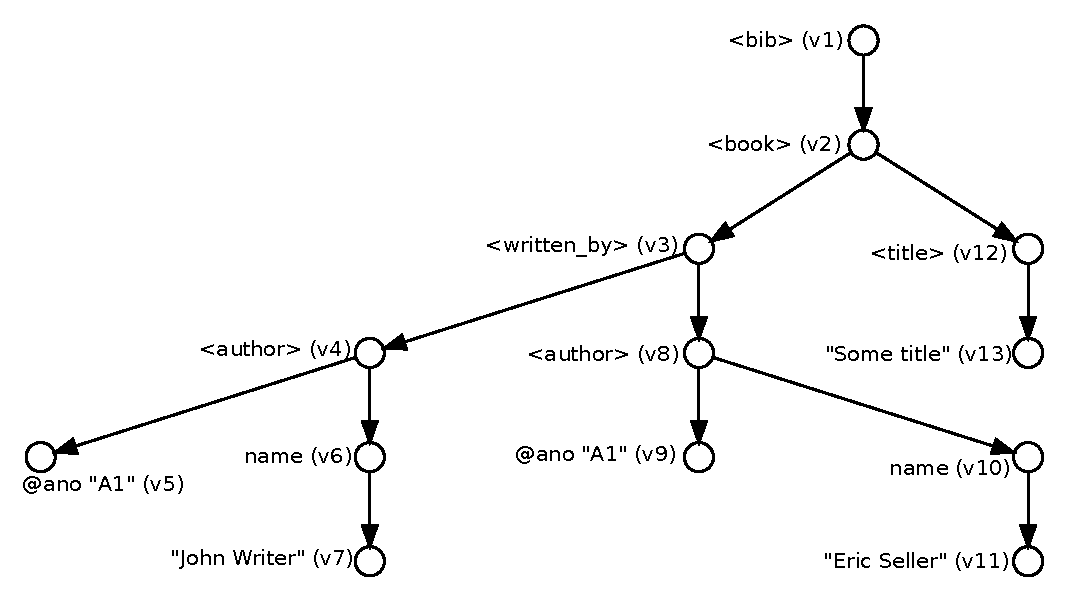
\includegraphics[scale=0.6]{nottuples1}}
    \subfloat[]{\label{nottuple2}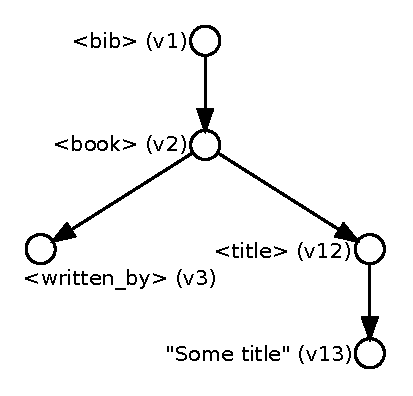
\includegraphics[scale=0.6]{nottuples2}}
	\caption[Two subtrees of the XML tree]{Two subtrees of the XML tree in Fig. \ref{example1} which are not tree tuples}
    \label{nottuples}
\end{figure}

In Fig. \ref{nottuple1}, the subtree is not a tree tuple, because the answer of the path $/bib/book/written\_by/author$ contains two distinct nodes (i.e. $v4$ and $v8$). The subtree in the Fig. \ref{nottuple2} is not a tree tuple, because it is not a maximal subtree (it is a subtree of a tuple from Fig. \ref{tuples}).\qed

\end{example}

\begin{define}[Functional Dependency]\label{fd1}
Being given a DTD $D$, a {\sl functional dependency} on $D$ is an expression of the form $S \rightarrow p$, where $S$ is a finite non empty subset of $paths(D)$ and $p \in paths(D)$.\qed
\end{define}

\begin{example}\label{fdExample}
Consider the XML tree in Fig \ref{example1}. The following functional dependency expresses the constraint that two distinct authors of the same book cannot have the same value of attribute \texttt{ano}:$$\{/bib/book, /bib/book/written\_by/author/@ano\} \rightarrow /bib/book/written\_by/author$$\qed
\end{example}

\subsection{Functional Dependency 2}

\begin{define}[Functional Dependency]\label{fd2}
With a given DTD $D$, a {\sl functional dependency} is of the form $\sigma = (P, P', (P_1, \dots, P_n \rightarrow P_{n+1}))$. Here $P$ is a  root path (path where the first element is a root element of an XML document), or $P = \epsilon$ (empty path). Each $P_i (i \in [1,n])$ is a singleton leaf path, and there is a no non-empty common prefix for $P_1, \dots, P_{n+1}$. Being given an XML document $T$ conforming to $D$, we say $T$ satisfies $\sigma$:iff $\forall v \in \{[\![P]\!]\}, \forall v_1, v_2 \in \{v[\![P']\!]\}$, if $v_1[\![P_i]\!] \equiv v_2[\![P_i]\!]$ for all $i \in [1,n]$, then $v_1[\![P_{n+1}]\!] \equiv v_2[\![p_{n+1}]\!]$.\qed
\end{define}

The main difference between two definitions of the functional dependency is that the former definition can use any path from $paths(D)$, whereas the latter considers that each $P_i (i \in [1,n])$ is from $StrPaths(D)$. That means the constraint from Example \ref{fdExample} cannot be expressed by functional dependency defined in \ref{fd2}, because of $/bib/book/written\_by/author$ path. Nevertheless, modified constraint from Example \ref{fdExample} expressed by FD defined in \ref{fd2} is shown in Example \ref{fd2Example}.

\begin{example}\label{fd2Example}
Consider the constraint $C$ saying that two distinct authors with different names of the same book cannot have the same value of attribute \texttt{ano}. The functional dependency expressing $C$ is defined as follows:

$$(bib/book, written\_by/author, (@ano \rightarrow name))$$\qed
\end{example}

\chapter{Analysis of Recent Approaches}

This chapter introduces description and categorization of recent approaches of repairing XML documents with usage of functional dependencies.

All approaches dealing with the problem of finding optimal repair can be divided into categories according to usage of elementary repair primitives. This repair primitives are: inserting node, deleting node, updating node and marking node as unreliable of XML document.

\section[Repairs and Consistent Answers for XML Data]{Repairs and Consistent Answers for XML Data with Functional Dependencies}

A technique for computing repairs which solves the problem of XML data inconsistency with respect to a set of functional dependencies was proposed in \cite{RepAndConsistentAnswer}. In this approach, the authors are trying to find a minimal set of update operations which makes XML data consistent. These update operations can be divided into two categories i) replacing a value associated with an element or an attribute, and ii) marking a particular node information as unreliable.

\subsection{XML Tree and Functional Dependency}

To be able to resolve problem of functional dependency violations in XML document, the authors try to introduce the concept of functional dependendenies based on those defined for relational databases. Concept of a tree tuple and functional dependency is defined in Definition \ref{treeTuple} and \ref{fd1}.

Given an XML tree $XT$ conforming a DTD $D$ and a functional dependency $F : S_1 \rightarrow S_2$ , we say that $XT$ satisfies $F (XT \models F )$ if for each pair of tree tuples $t_1, t_2$ of $XT$, $t_1.S_1 = t_2.S_1 \land t_1.S_1 = \emptyset \Rightarrow t_1.S_2 = t_2.S_2$ . Given a set of functional dependencies $\mathcal{FD} = \{F_1 , \dots, F_n\}$ over $D$, we say that $XT$ satisfies $\cal FD$ if it satisfies $F_i$ for every $i \in 1..n$.

\subsection{Repairing inconsistent XML data}

Authors of this approach chose two kinds of actions to repair inconsistent XML data with regard to functional dependencies. The first action is updating the value of an attribute or content of an element. As the second action authors choose marking inconsistent element as "unreliable" rather than deleting it, because removing elements from an XML document leads to some undesired drawbacks: it does not always suffice to remove inconsistency and deleting a node can lead to a new document not valid against the given schema.

Depending on XML data and defined functional dependencies, each inconsistency could have many possible strategies to repair it. From all the possible repair strategies, the authors prefer those, for which smaller changes are made to the original document.

\begin{example}
Consider XML tree $XT$ from Example \ref{example1ref} conforming the DTD $D$ defined below, which is representing collection of books and the following functional dependency:\\ $\{bib.book, bib.book.written\_by.author.@ano\} \rightarrow bib.book.written\_by.author$.
\begin{verbatim}
<!ELEMENT bib (book+)>
<!ELEMENT book (written_by, title)>
<!ELEMENT written_by (author+)>
<!ELEMENT author (name)>
<!ATTLIST author ano CDATA>
<!ELEMENT name PCDATA>
<!ELEMENT title PCDATA>
\end{verbatim}
The functional dependency defined above requires that for each book, there is only one element author having a given $@ano$ value. Therefore $XT$ does not satisfy the given functional dependency, because two author elements of the same book have the same value of attribute $@ano$. To resolve this data inconsistency, we can use two different repair strategies: 1) changing one of the value of attribute $@ano$; 2) marking one of the element author as unreliable. Since the first strategy changes only attribute $@ano$, it is preferred to second strategy, which changes a larger portion of document, since it marks whole author element as unreliable.
\qed
\end{example}


\subsection{Repair Algorithm}

Before introducing the algorithm to repair inconsistent XML document, let us define reliability of elements in XML tree:

\begin{define}[R-XML Tree]
A R-XML $tree$ is a triplet $RXT = \langle T, \delta, \varrho \rangle$, where $\langle T, \delta \rangle$ is an XML tree and $\varrho$ is a reliability function from $N_T$ to \texttt{\{true, false\}}, such that, for each pair of nodes $n_1 , n_2 \in N_T$ with $n_2$ descendant of $n_1$, it holds that $\varrho(n_1) = false \Rightarrow \varrho(n_2) = false$.\qed
\end{define}

To be able to create a repair, R-XML Tree must not satisfy FD according to definition of weak satisfiability:

\begin{define}[Weak satisfiability]
Let $RXT = \langle T, \delta, \varrho \rangle$ be an R-XML tree conforming a DTD $D$, and $f: S \rightarrow p$ be a functional dependency. We say that $RXT$ weakly satisfies $f$ ($RXT \models_w f$) if one of the following conditions holds:
\begin{enumerate}
	\item $\langle T, \delta \rangle \models f$;
    \item for each pair of tuples $t_1$, $t_2$ of $RXT$ one of the following holds:
    \begin{enumerate}
    	\item there exists a path $p_i \in S$ such that: \\
$(\varrho(p_i(t_1)) = false) \lor (\varrho(p_i(t_2)) = false)$;
        \item $(\varrho(p(t_1)) = false) \lor (\varrho(p(t_2)) = false)$.\qed
    \end{enumerate}
\end{enumerate}
\end{define}

The repair of an R-XML tree which not satisfies $\mathcal{FD}$ set of functional dependencies is a pair of functions $\delta'$ and $\varrho'$ such that $RXT'$ tree composed of the original tree and the repair ($RXT' = \langle T, \delta' \cdot \delta, \varrho' \cdot \varrho \rangle$) weakly satisfies FD ($RXT' \models_w \mathcal{FD}$).\\
With a repair $\langle \delta, \varrho \rangle$ of R-XML tree and a set of labelled nodes $N$ of this tree, we denote with $Update_{\delta}(N)$ the set of nodes modified by $\delta$. Analogously, we denote $True_{\varrho}(N) = \{n \in N| \varrho(n) = true\}$ and $False_{\varrho}(N) =\{n \in N | \varrho(n) = false\}$.

\begin{define}[Minimal Repair]
Let $RXT = \langle T, \delta, \varrho \rangle$ be an R-XML tree conforming DTD $D$, $\mathcal{FD}$ a set of functional dependencies and $R_1 = \langle \delta_1, \varrho_1 \rangle$, $R_2 = \langle \delta_2, \varrho_2 \rangle$ two repairs for $RXT$. We say that $R_1$ is smaller than $R_2$ ($R_1 \preceq R_2$) if $Updated_{\delta_1}(N_T)\ \cup\ False_{\delta_1}(N_T) \subseteq Updated_{\delta_2}(N_T)\ \cup\ False_{\delta_2}(N_T)$ and $False_{\delta_1}(N_T) \subseteq False_{\delta_2}(N_T)$. Repair $R$ is minimal if there is no repair $R' \neq R$ such that $R' \preceq R$.\qed
\end{define}

An R-XML tree is used as an input for the main algorithm computing repaired R-XML tree described in Algorithm \ref{repAlgo}. First the algorithm computes all the possible repairs of tuples which not satisfy a functional dependecy using the function \texttt{computeRepairs} (lines 2-6). Next all non-minimal repairs are removed from all possible repairs (line 7). In the last step, all the repairs are merged and a unique repaired R-XML tree is returned.

\begin{algorithm}[H]
\caption{XML Repair}
\label{repAlgo}
\begin{algorithmic}[1]
\REQUIRE{\ \\
$RXT = \langle T, \delta, \varrho \rangle$: R-XML tree conforming a DTD $D$\\
$\mathcal{FD} = {F_1, \dots, F_m}$: Set of functional dependencies}
\ENSURE a unique repaired R-XML tree

\STATE $S = \emptyset$ \COMMENT Set of repairs
\FORALL{$(F: S \rightarrow p) \in \mathcal{FD}$ s.t. $RXT \not \models_w F$}
	\FORALL{$t_1, t_2$ tuples of $RXT$ s.t. $t_1, t_2$ do not weakly satisfy $F$}
		\STATE $S = S \cup computeRepairs(F, t_1, t_2, RXT)$
	\ENDFOR
\ENDFOR
\STATE $S = removeNonMinimal(S, RXT)$
\STATE $\langle \delta', \varrho' \rangle = mergeRepairs(S)$
\RETURN $\langle T, \delta' \cdot \delta, \varrho' \cdot \varrho \rangle$
\end{algorithmic}
\end{algorithm}

Function \texttt{computeRepairs}(in algorithm \ref{computeRepairs}) gets R-XML tree, a functional dependency $F$ and a tuples $t_1, t_2$ of R-XML tree as input and computes the repair as follows:
\begin{itemize}
	\item If path $p$ denotes a textual element, one of the two terminal values of $t_1.p$ or $t_2.p$ is changed, so that they become equal (line 3).
	\item Otherwise $p$ denotes a node, so either the node $t_1.p$ or $t_2.p$ is marked as unreliable (line 5).
	\item For each path $p_i$ of the left side of a functional dependency $F$
	\begin{itemize}
		\item If path $p_i$ denotes a textual element, then one of the two terminal values $t_1.p_i$ or $t_2.p_i$ is changed to the new generated value ($\perp$) (line 9).
		\item Otherwise $p_i$ denotes a node, so one of the nodes $t_1.p_i$ or $t_2.p_i$ is marked as unreliable (line 11).
	\end{itemize}
\end{itemize}

\begin{algorithm}[H]
\floatname{algorithm}{Function}
\caption{$computeRepairs(F, t_1, t_2, RXT)$}
\begin{algorithmic}[1]\label{computeRepairs}
\REQUIRE{\ \\
$RXT = \langle T, \delta \varrho \rangle$: R-XML tree conforming a DTD $D$\\
$F: X \rightarrow p$ functional dependency\\
$t_1, t_2$ tuples of $RXT$}
\ENSURE $S$: Set of repairs

\STATE $S = \emptyset$
\IF{$p \in StrPaths(D)$}
	\STATE $S = S \cup \{\langle \{\delta(p(t_1)) = t_2.p\}, \varrho \rangle\} \cup \{\langle \{\delta(p(t_2)) = t_1.p\}, \varrho \rangle\} $
\ELSE
	\STATE $S = S \cup \{\langle \emptyset, \varrho_{\{t_1.p\}} \cdot \varrho \rangle\} \cup \{\langle \emptyset, \varrho_{\{t_2.p\}} \cdot \varrho \rangle\}$
\ENDIF
\FORALL{$p_i \in X$}
	\IF{$p_i \in StrPaths(D)$}
		\STATE $S = S \cup \{\langle \{\delta(p_i(t_1)) = \perp_1\}, \varrho \rangle\} \cup \{\langle \{\delta(p_i(t_2)) = \perp_2\}, \varrho \rangle\}$
	\ELSE
		\STATE $S = S \cup \{\langle \emptyset, \varrho_{\{t_1.p_i\}} \cdot \varrho \rangle\} \cup \{\langle \emptyset, \varrho_{\{t_2.p_i\}} \cdot \varrho \rangle\}$
	\ENDIF
\ENDFOR
\RETURN $S$
\end{algorithmic}
\end{algorithm}

\subsection{Conclusion}

The authors proposed a technique for repairing XML documents violating functional dependencies based on approaches proposed for relational database repairing. The algorithm introduces two possible repair primitives, which creates many possible result from which those with minimal impact on document are chosen. However the authors not consider creation of new violations after repairing the initial violations as it is in \cite{ImprovingXML}. Another disadvantage of this approach is that a unnecessary repair of some particular violation could be applied to an XML document because another repair could repair that violation before.

\section{Querying and Repairing Inconsistent XML Data}

Studying the problem of repairing inconsistent XML documents with respect to a set of functional dependencies and investigating the existence of repairs has been introduced in \cite{QueryXML}. Authors introduce two kind of repair primitives. The first is deleting "unreliable" nodes of document and the second is inserting a new nodes. Similarly to another approaches, authors prefer minimal set of repair primitives applied to the XML document to form a repair.

The introduced repair primitives the authors use in three different repair strategies consisting of:
\begin{enumerate}
	\item \textit{(general) repairs}, where both delete and insert operations are used,
	\item \textit{cleaning repairs}, where for documents interpreted as "dirty" only delete operations are used to repair inconsistencies,
	\item \textit{completing repairs}, where for documents interpreted as incomplete, insert operations are used.
\end{enumerate}

\subsection{General Repair}

With the insert and delete operations as repair primitives, is updated the structure of the XML document which conforms DTD $D$ (defined in Definition \ref{dtdDef}) and violated functional dependency. The insert operation is represented as $\langle  + [x]a[y], z\rangle$, where i) $x$ is a node identifier, ii) $a$ is a label, iii) $y$ is either a node identifier or a value ($y$ is a value, if $a \in \alpha \cup \{S\}$; otherwise it is a node identifier), and iv) $z$ denotes the child of $x$ which must immediately precede $y$ ($\perp$ if $y$ is inserted as the first or a single child of $x$). The deletion is represented as $-[x]a[y]$, where $x$ is a node identifier, $a \in \alpha \cup \tau \cup \{S\}$, and $y$ is either a node $id$ or a string value, denoting the node to be deleted.\\
The set $R$ of update operations can be divide into two subsets: $R^+$ is a the subset of all the insertion operations in $R$; $R^-$ is the subset of all the deletion operations. A set $R$ is said to be consistent if the following conditions are hold:
\begin{enumerate}
	\item the deletion of node implies the deletion of all descendant nodes;
    \item insertions cannot refer to deleted nodes.
\end{enumerate}
We say that two sets of update operations $R_1$ and $R_2$ are equivalent ($R_1 \equiv R_2$) if $R_1$ is equal to $R_2$ up to an injective renaming of node identifiers. Moreover, we say that $R_1 \preceq R_2$ if $R_1^- \subseteq R_2^- \lor R_1^- = R_2^-$ and $R_1^+ \subseteq R_2^+$. We say that $R_1 \sqsubseteq R_2$ if there exists a $R_2' \equiv R_2$ such that  $R_1 \preceq R_2'$. At last $R_1 \sqsubset R_2$ if $R_1 \sqsubseteq R_2$ and $R_1 \not \equiv R_2$.\\

With defined basic repair operations for general repair of inconsistent XML document let us define a repair as follows:

\begin{define}[Repair]
Given an XML tree $T$, a DTD $D$ and a set of integrity constraints $IC$(definition \ref{integConstr}), a set of update operations $R$ is said to be a repair of $T$ (with respect to $D$ and $IC$) if $R(T) \models IC$, where $R(T)$ is application of consistent set of updates $R$ to $T$, $R(T)$ conforms $D$ and $\not \exists R' \sqsubset R$ such that $R'(T) \models IC$ and $R'(T)$ conforms $D$.
\end{define}

With further investigation, the authors discover that the problem of deciding whether there exists a repair for a XML document in the presence of DTD with functional dependencies is undecidable. Therefore they consider restricted forms of repairs, more specifically cleaning and completing repairs.

\subsection{Conclusion}

In this approach the authors introduce different types of repairs (general, cleaning and completing) and focus on checking whether exists a repair for many classes of integrity constraints (general integrity constraints, inclusion dependencies, functional dependencies, etc.). For the functional dependencies the authors found out that the problem of checking whether there exists a general repair for an XML document is $\mathcal{NP}$-complete.


\section{Improving XML Data Quality with Functional Dependencies}

The algorithm for repairing XML functional dependency violations which uses modification of node value as the repair primitive has been proposed in \cite{ImprovingXML}. For finding the optimal repair of an XML document, the authors introduce a cost model, which assign a weight to each leaf node in an XML document. The optimal repair is the one with the lowest repair cost which is measured by the total weight of the modified nodes.

The authors of the approach found out that repairing one functional dependency violation can violate another. Therefore they divide the main algorithm into two phases. In the first phase, the conflict hypergraph capturing the initial functional dependency violations is constructed, and all the violations are fixed by modifying the values of all the nodes on a vertex cover of the conflict hypergraph. In the second phase, remaining violations are resolved by modifying the violating nodes and their core determinants to prevent of introducing new conflicts.

\subsection{Cost Model and Repairing Primitive}

Each leaf node $v$ of XML tree is associated a weight from range $[0,1]$, which is denoted $W(v)$. Let us assume that the larger the weight of the leaf the more reliable it is. The weight may be automatically generated by statistical methods or it can be assigned by a user.

As was mentioned earlier, a repairing primitive is a node value modification, where for repairing algorithm a combination of two rules to resolve violation is used. Let us have a $FD$ $\sigma = (P, P', (P_1, \dots, P_n \rightarrow P_{n+1}))$ (from Definition \ref{fd2}) and consider two nodes $v_1$ and $v_2$ matching path $P'$ in a subtree rooted at a node in $\{[\![p]\!]\}$. If the child nodes of $v_1$ and $v_2$ qualified by paths $P_i$ have equal values for all $i \in [1,n]$ and their child nodes qualified by $P_{n+1}$ have different values, then $v_1$ and $v_2$ violates $\sigma$. The first rule used to repair this violation is to change the value of the node qualified by $P_{n+1}$ from $v_1$ to the value of $v_2$'s child node that matches $P_{n+1}$(or reversely). The second rule is to choose an arbitrary $P_i (i \in [1,n])$, and introduce a new value to the node qualified by $P_i$ from $v_1$ (or $v_2$).

\begin{define}[Optimal repair]
Given an inconsistent XML document $T$ violating a set $\Sigma$ of $FD$s, the repair $T_R$ of $T$ is called optimal repair, if $T_R$ has the minimum cost among all repairs of $T$. The cost $cost(T_R)$ is defined as:
\begin{displaymath}
cost(T_R) = \sum_{v \in T} w(v) \times dist(v, v_R),
\end{displaymath}
where $dist(v, v_R)=1$ if $val(v) \neq val(v_R)$, otherwise $dist(v, v_R)=0$.\qed
\end{define}

\subsection{Initial Conflicts Hypergraph}

A weighted hypergraph is used in the first part of repair algorithm as a tool modeling initial functional dependency violations in an XML document. Hypergraph $g$ of XML document $T$ can be defined as a pair $g = (V,E)$, where $V$ stands for a set of elements (called nodes), and $E$ is a set of non-empty subset of $V$ called hyperedges, more accurately each hyperedge indicates a set of value nodes violating FDs. Since hypergraph is weighted and a cost model is used in this approach, each node $v \in V$ of the hypergraph is assigned with a weight $w(v)$, which is the same as the weight of $v$ in $T$.\\

To actually resolve the problem of repairing FD violations in an XML document, the authors convert this problem into well-known problem of weighted vertex cover for hypergraph \cite{ApproxAlgo}. Let us have hypergraph $g = (V,E)$, where each hyperedge $e \in E$ is a set of value nodes which violate some FD. In a repair of an inconsistent XML document, for each hyperedge at least one value node is modified, therefore it is essential to find a vertex cover (VC) for $g$, which is a set $S \subseteq V$, such that for all edges $e \in E$, $S \cap e \neq \emptyset$. Since the hypergraph is weighted, we can define weight of VC as the total weight of all vertices in $S$.\\

The algorithm fixing initial FD violations is shown in Algorithm \ref{fixInit}. The algorithm uses approximation algorithm to find VC for the minimum weighted vertex cover proposed in \cite{ApproxAlgo}.

\begin{algorithm}
\caption{Fix-Initial-Conflicts}
\label{fixInit}
\begin{algorithmic}[1]
\REQUIRE An XML document T, a set $\Sigma$ of FDs.
\ENSURE A modified document T.
\STATE Create the initial conflict hypergraph $g$ of $T$ w.r.t $\Sigma$
\STATE Use a known algorithm to find an approxiamtion $VC$ for the minimum weighted vertex cover of $g$
\STATE $remaining$ := VC
\WHILE{There are two target nodes $v_1, v_2 \in T$ violating a FD $\sigma \in \Sigma$, and $v_1[\![P_{n+1}]\!]$ or $v_2[\![P_{n+1}]\!]$ is the only node in VC from the set of nodes $\{v_1[\![P_i]\!](i \in [1, n+1])\} \cup \{v_2[\![P_i]\!](i \in [1, n+1])\}$. (W.l.o.g assume the violation is as follows: $\sigma = (P,P',(P_1,\dots,P_n \rightarrow P_{n+1}))$, $v \in \{[\![P]\!]\}$, $v_1, v_2 \in \{v[\![P']\!]\}$, $v_1[\![P_i]\!] \equiv v_2[\![P_i]\!]$ for all $i \in [1,n]$, and $v_1[\![P_{n+1}]\!] \not \equiv v_2[\![P_{n+1}]\!]$.)}
\STATE $val(v_1[\![P_{n+1}]\!])$ := $val(v_2[\![P_{n+1}]\!])$ \COMMENT W.l.o.g, we assume $v_1[\![P_{n+1}]\!]$ is in VC
\ENDWHILE
\FORALL{node $u \in remaining$}
\STATE $val(u)$ := $gen\_new\_value()$
\STATE \COMMENT Introduce new values to all the remaining nodes in VC
\ENDFOR
\end{algorithmic}
\end{algorithm}

\subsection{Resolving Violations Thoroughly}

After repairing initial FD violations, there is a chance that new violations may be introduced, therefore the authors provided a method to do modifications on value nodes without incurring new conflicts (Algorithm \ref{fixRest}). This method uses core determinant $C_u$ of value node $u$ defined as follows:

\begin{define}[Core Determinant]
Given an XML document $T$, a set $\Sigma$ of FDs and a node $u$ in $T$, we say that a set of nodes $\{u_1, u_2, \dots, u_n\}$ is a $\sigma\!-\!determinant$ of $u$, if there exists a nontrivial FD $\sigma = (P, P', (P_1, \dots, P_n \rightarrow P_{n+1}))$ logical implied by $\Sigma$, such that $\exists v \in \{[\![P]\!]\}, \exists v_1 \in \{[\![P']\!]\}, v_1[\![P]\!] = u_i$ for $i \in [1,n]$, and $v_1[\![P_{n+1}]\!] = u$.\\
We say that a set $C_u$ of nodes is a core determinant of $u$, if (a) for every nontrivial FD $\sigma$ implied by $\Sigma$ and every set $W$ that is $\sigma\!-\!determinant$ of $u$, $C_u \cap W \neq \emptyset$; and (b) for any proper subset $C_u'$ of $C_u$, there exists a nontrivial FD $\sigma$ implied by $\Sigma$, and a set $W$ that is $\sigma\!-\!determinant$ of $u$, $C_u' \cap W = \emptyset$.\qed
\end{define}

\begin{algorithm}[H]
\caption{Resolve-Remaining-Violations}
\label{fixRest}
\begin{algorithmic}[1]
\REQUIRE An XML document T, a set $\Sigma$ of FDs.
\ENSURE A modified document T, with all the violations fixed.

\WHILE{there are FD violations in T w.r.t. $\Sigma$}
\STATE pick a violating value node $u$ from T w.r.t. $\Sigma$
\STATE let $C_u$ be a core determinant $u$
\FORALL{node $w \in (C_u \cup \{u\})$}
\STATE $val(w)$ := $gen\_new\_value()$
\STATE \COMMENT it guarantees that no new violations will be introduced
\ENDFOR
\ENDWHILE
\end{algorithmic}
\end{algorithm}

\subsection{Conclusion}

The authors introduced effective two-step heuristic method to solve a problem of finding optimal repair of XML violations against functional dependencies, which is $\mathcal{NP}$-complete. Moreover, they experimentally verified the efectivity and scalability of their approach using real-life and synthetic data.

\chapter{Proposed Algorithm}\label{kap4}

The main goal of this thesis is to propose an algorithm to repair an XML document violating functional dependencies defined for this document. We use an XML tree and tree tuples to represent XML data. We would like our algorithm to have the following features::

\begin{itemize}
	\item Incorporation of a weight model into the XML data representation to provide the selection of repair candidates with the lowest modification cost.
    \item Involvement of a user in the process of finding and applying repair candidates.
    \item Application of a single repair candidate at the time and then recalculate repair candidates again to prevent using unnecessary repairs to repair one violation and also to prevent of introducing new violations, which will not be repaired.
    \item The paths which form a functional dependency are described with XPath language \cite{xpath}, where only paths with basic construction are allowed (only path constructed with "/", "//" or "@", no wildcards, "[]" or another constructs are allowed).
    \item We introduce a new concept of the so-called repair group, which clusters repair candidates (repairs for repairing one FD violation) repairing the same violation, or modifying the same part of the XML tree.
\end{itemize}


\section{Repairing Algorithm}

The proposed algorithm is based on the algorithm described in \ref{RepConstAnswers} presented in \cite{RepAndConsistentAnswer}. This algorithm was chosen because of simple representation of the XML data using a concept which corresponds with concept used in relational databases. Another reason, besides modification of node value as an update operation, is using also marking particular node information as unreliable, which can reveal forgotten inconsistencies in the data.

\begin{algorithm}
\caption{Repair RW-XML tree}
\label{propAlgo}
\begin{algorithmic}[1]
\REQUIRE{\ \\
$RXT = \langle RT, \omega \rangle$: RW-XML tree conforming to DTD $D$\\
$\mathcal{FD} = {F_1, \dots, F_m}$: Set of functional dependencies}
\ENSURE a unique repaired RW-XML tree

\STATE $resultRXT = RXT$
\WHILE{$resultRXT \not \models_w \mathcal{FD}$}
    \STATE $S = \emptyset$ \COMMENT Set of repair groups
    \FORALL{$(F: S \rightarrow p) \in \mathcal{FD}$ s.t. $RXT \not \models_w F$}
    	\FORALL{$t_1, t_2$ tuples of $RXT$ s.t. $t_1, t_2$ do not weakly satisfy $F$}
		    \STATE $S = S \cup computeRepairGroup(F, t_1, t_2, RXT, S)$
	    \ENDFOR
    \ENDFOR

    \STATE $R = getRepair(S, RXT)$
    \STATE $resultRXT = applyRepair(R, resultRXT)$
\ENDWHILE

\end{algorithmic}
\end{algorithm}

The algorithm is split into three steps, where the second and the third step are repeated until all violations are repaired. In the first step, XML document and FDs are loaded, and XML tree with corresponding tree tuples are created. Next step of the algorithm computes repair groups containing repair candidates for FD violations. In the third step the chosen repair candidate is applied to an XML tree. In Algorithm \ref{propAlgo} we can see the simplified process of repairing XML FD violations, which covers the second and the third step of the whole algorithm.

\subsection{Initial data model}

To represent an XML document we use an extended R-XML tree (Definition \ref{rxmlTree}), called RW-XML tree, which has weights assigned to each node of the tree. The weight of a node is from interval $[0,1]$ and indicates correctness of the data the particular node holds, meaning the higher the weight is, the more correct that particular node is. The weights are used to measure the cost of repair candidates, where candidate with the lowest cost is picked to be applied to the XML tree. This is also the first place where some kind of user interaction can be implemented. The user could assign the weights to nodes manually or could use some sort of statistical methods to generate them automatically. If the user does not assign weights nor does he use statistical methods, a default weight is assigned to all nodes.

\begin{example}
Consider the XML document and corresponding XML tree from Example \ref{example1}. Let us assign weights to nodes defined by XPath constructs shown in Table \ref{weightTab}. The XML tree with assigned custom and also default weights is shown in Fig. \ref{weightsFig}.

\begin{table}[h]
\begin{tabular}{r | c}
XPath & weight\\\hline
$/bib/book/title/text()$ & 0.8\\
$/bib/book/written\_by/author$ & 0.6\\
$/bib/book/written\_by/author/@ano$ & 0.1\\
\end{tabular}
\caption{Table of custom weights assigned to the XML tree.}
\label{weightTab}
\end{table}

\begin{figure}[H]
    \centering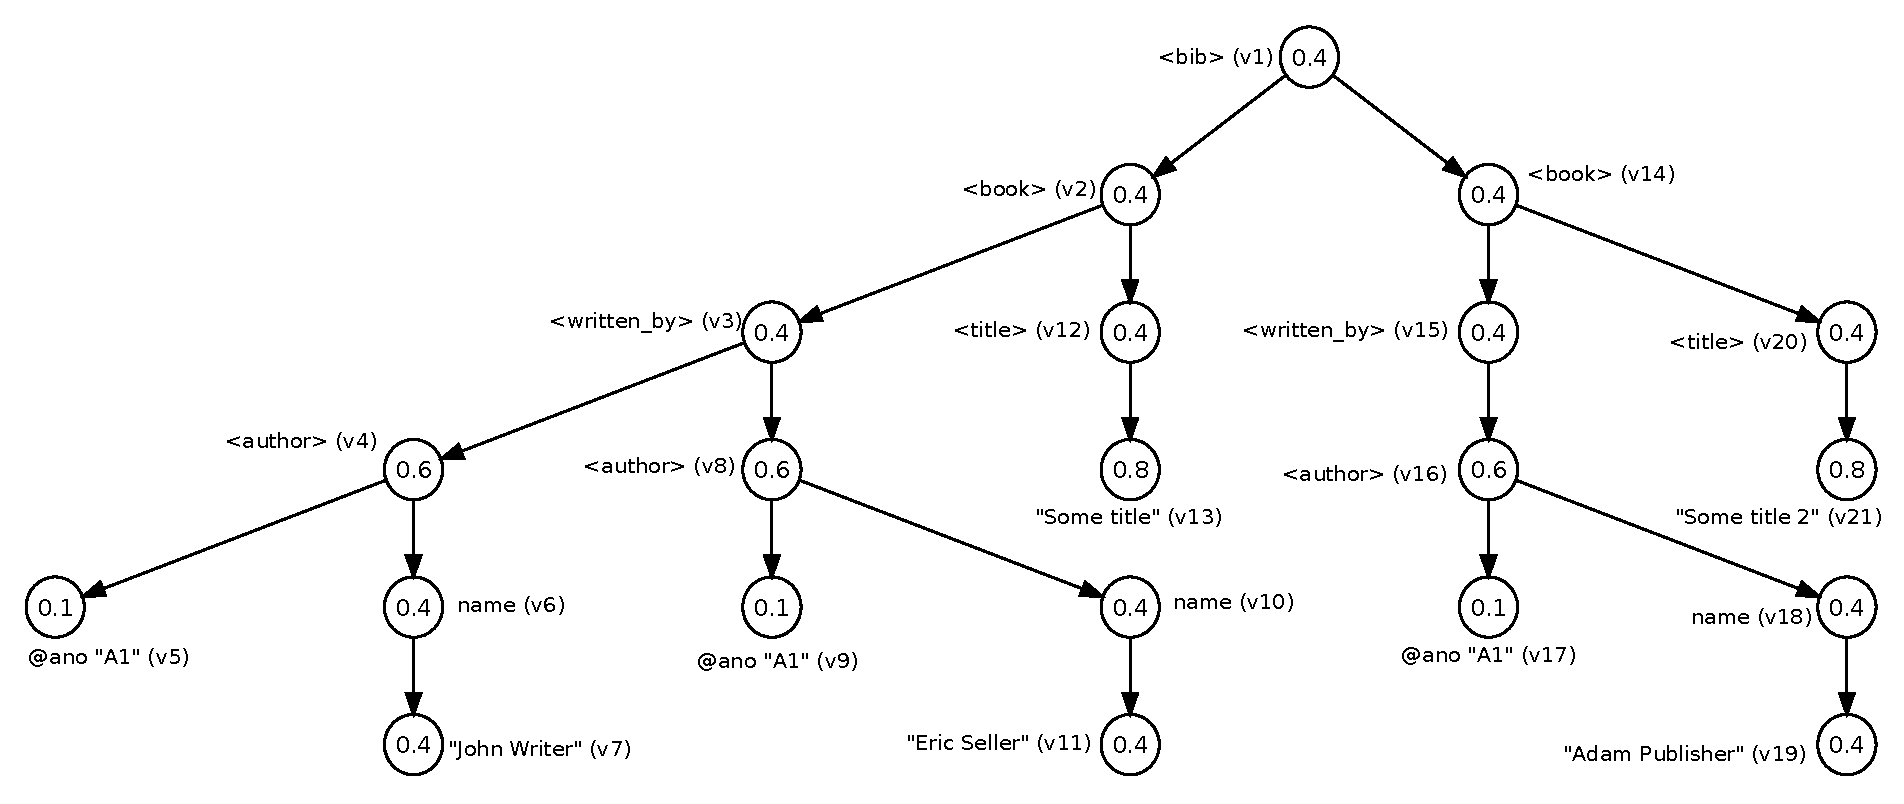
\includegraphics[width=\textwidth]{weights}
	\caption{The XML tree with assigned weights to the nodes.} \label{weightsFig}
\end{figure}
\qed
\end{example}


\begin{define}[RW-XML tree]
A {\sl RW-XML tree} is a pair $RWXT = \langle RXT, \omega \rangle$, where $RXT$ is an R-XML tree and $\omega$ is a weight function from $N_T$ to $[0,1]$.\qed
\end{define}

After creating the RW-XML tree from input XML data, a set of tree tuples (defined in Definition r\ref{treeTuple}) is constructed. Since the set $paths(D)$, containing all possible paths defined in DTD $D$, can be infinite (DTD can define recursive structure of elements), the actual content of $paths(D)$ is modified to reflect the current structure of the RW-XML tree. Since definition of a tree tuple says that answer to the path $p$ contains at most one element, our modification of $paths(D)$ has no effect on constructing tree tuples if a DTD defines some optional path which is not defined for the RW-XML tree $RWXT$ (the set $p(RWXT)$ is empty).

Functional dependencies as defined in Definition \ref{fd1} consist of paths described with XPath. As was described before, these paths can only have basic structure shown in Example \ref{pathsExample}.

\begin{example}\label{pathsExample}
Example of paths that can be used in functional dependencies:
\begin{verbatim}
//bib/book/author
/bib/book/author/@ano
/bib/book/author/name/text()
\end{verbatim}
\end{example}

\subsection{Computing Repair Groups}

With RW-XML tree $RWXT$ and corresponding tree tuples from input data created, we can now proceed to compute repair groups. Repair group is a set of repair candidates, which repairs the same FD or modifies the same part of $RWXT$. Each repair candidate is a pair of functions $\delta$ and $\varrho$ ($\langle \delta, \varrho \rangle$), which either modifies value of an RW-XML tree node ($\delta$ is defined) or marks a node as unreliable ($\varrho$ is defined). The $\delta$ function of a repair candidate is defined the same way as in the XML tree (Definition \ref{xmlTree}) and defines a new value of the RW-XML tree node. Similarly, the $\varrho$ function defines the node which is marked as unreliable.

To be able to compute repair groups, we need to decide which FDs violate $RWXT$. This can be achieved by finding all tree tuple pairs that do not weakly satisfy particular FD (Definition \ref{weakSatisf}). A repair group is then computed for each tuple pair (line 6 in Algorithm \ref{propAlgo}).

The function \texttt{computeRepairGroup()} responsible for creating the repair group is shown in Algorithm \ref{repairGroupAlgo}. The function gets an RW-XML tree, a functional dependency $F$, tuples $t_1$, $t_2$ and a set of repair groups $RGS$ and computes the repair group containing repair candidates as follows:

\begin{enumerate}
	\item First the repair candidates are created using function \texttt{computeRepairs()} from Algorithm \ref{repAlgo} (line 1). Since an R-XML tree is a special case of RW-XML tree where all the weights are equal to zero, we can pass RW-XML tree as a parameter to this function.
    \item Next a check is performed whether the repair candidates intersect other candidates from existing repair groups (line 2)
    \begin{itemize}
    	\item If the candidates intersect with some group, they are added to this group (line 3)
        \item Otherwise a new repair group containing repair candidates is created (line 5)
    \end{itemize}
\end{enumerate}

\begin{algorithm}
\floatname{algorithm}{Function}
\caption{$computeRepairGroup(F, t_1, t_2, RXT, RGS)$}
\label{repairGroupAlgo}
\begin{algorithmic}[1]
\REQUIRE{\ \\
$RXT = \langle T, \omega \rangle$: RW-XML tree conforming to DTD $D$\\
$F: X \rightarrow p$ functional dependency\\
$t_1, t_2$ tuples of $RXT$\\
$RGS$ set of repair groups}
\ENSURE $RG$: repair group

\STATE $S = computeRepairs(F, t_1, t_2, RXT)$ \COMMENT set of repair candidates

\IF{$candidatesIntersectRepairGroups(S, RGS)$}
\STATE $RG = getIntersectingRepairGroup(S, RGS)$
\ELSE
\STATE $RG = createNewRepairGroup(S)$
\ENDIF

\RETURN $RG$
\end{algorithmic}
\end{algorithm}

Example \ref{repairExample} demostrates repair candidates of one repair group modifying node values and marking nodes as unreliable.

\begin{example}\label{repairExample}
Consider XML data and functional dependency from Example \ref{fdrepairExample}, where XML data is graphically represented as XML tree $XT$ in Fig \ref{example1}. The $XT$ violates FD $$\{/bib/book, /bib/book/written\_by/author/@ano\} \rightarrow /bib/book/written\_by/author$$ because two authors of the same book have the same value of attribute $@ano$. One repair group with these repair candidates is created:
\begin{itemize}
	\item $R_1 = \langle \{\delta(v5) = \perp\},\varrho_{\{\}}(v) \rangle$
    \item $R_2 = \langle \{\delta(v9) = \perp\},\varrho_{\{\}}(v) \rangle$
    \item $R_3 = \langle \{\},\varrho_{\{v4,v5,v6,v7\}}(v) \rangle$
    \item $R_4 = \langle \{\},\varrho_{\{v8,v9,v10,v11\}}(v) \rangle$
    \item $R_5 = \langle \{\},\varrho_{\{v2,v3,\dots,v13\}}(v) \rangle$
\end{itemize}

First two repair candidates modify the value of an attribute $@ano$ by assigning newly generated value ($\perp$). Next two repair candidates mark each \emph{author} node with its child nodes that have the same $@ano$ attribute respectively. The last candidate marks as unreliable a whole subtree with the \emph{book} node holding \emph{authors} with the same attribute as the root node.\qed
\end{example}

\subsubsection{Weight model of a Repair Group}

In this section, we introduce a weight model for a repair group, which will be used in the next step of our repair algorithm. Before we define a weight of a repair group, let us introduce some important notations.

Being given a repair candidate $R$, $Modified_\delta(R)$ denotes the set of nodes modified by $\delta$ function from $R$. Analogously, we denote $Modified_\varrho(R)$ the set of nodes modified by $\varrho$ function. The count of nodes modified by repair candidate $R$ is denoted with $\lambda(R)$. Last, we denote $PS(R)$ a set of paths defining all nodes modified by $R$ (example of the set $PS(R)$ is shown in Example \ref{PSExample}).

\begin{example}\label{PSExample}
Consider the XML tree from Fig. \ref{example1} and a repair candidate, which marks nodes $v12$ and $v13$ as unreliable. Then the set $PS(R)$ contains the following paths:
\begin{verbatim}
/bib/book/title
/bib/book/title/text()
\end{verbatim}\qed
\end{example}


Since each repair candidate consists of a set of nodes which are modified (marked as unreliable or having a modified value), we can compute the cost of each candidate. It is important to say that unlike in original approach, we do not prefer repair candidates that modify the value of the nodes to those marking nodes as unreliable. Therefore we added a coefficient $k$ to the calculation of the repair candidate cost, so that the priority of repair candidate marking node as unreliable can be achieved. The definition of repair candidate cost is as follows:

\begin{define}[Repair Candidate Cost]
Being given an RW-XML tree $RXT$ and a repair candidate $R$, we define the cost of $R$ as:
$$cost(R) = \sum_{u \in Modified_\delta(R)} \omega(u) + \sum_{v \in Modified_\varrho(R)} \omega(v) \cdot k,$$
where $k$ is the priority of repairing the candidate by modifying the node value in constrast to marking it unreliable.\qed
\end{define}

By default, $k$ is set to such value that the cost of repair candidate marking as an unreliable node will be higher than the one that modifies node value. However, this is another place where user can intervene and change the priority of repair candidates. We show in Example \ref{koefK} how $k$ can change the costs of repair candidates.

\begin{example}\label{koefK}
Consider XML tree $XT$ and repair candidates from Example \ref{repairExample}. The default weight of all nodes $v$ of $XT$ is $\omega(v) = 0.5$. If the coefficient $k = 1$, cost of repair candidates would be as follows: $cost(R_1) = 0.5$, $cost(R_2) = 0.5$, $cost(R_3) = 2$, $cost(R_4) = 2$ and $cost(R_5) = 6$.
Let us assume that a repair candidate with the lowest repair cost will be applied to $XT$. If we order costs of repair candidates from the lowest to the highest, we can see that candidates which have marked unreliable nodes are in the end (and will not be applied to $XT$).

However, if we set the coefficient $k = 0.1$, costs of candidates would be sorted as follows: $cost(R_3) = 0.2$, $cost(R_4) = 0.2$, $cost(R_1) = 0.5$, $cost(R_2)  = 0.5$ and $cost(R_5) = 0.6$. We can see that order of costs has significantly changed and the candidate which will be applied is $R_3$ (marking nodes as unreliable).\qed
\end{example}

And, finally, since a repair group is a set of repair candidates, its weight can be defined as follows:

\begin{define}[Repair Group weight]
Being given an RW-XML tree $RXT$ and a repair group $RG$, we define the {\sl weight} of $RG$ as the sum of costs of all repair candidates in the $RG$.
\end{define}

\subsection{Repair Candidate Selection and Application}

The last step of our algorithm can be divided into two parts, namely selection of the repair candidate and the subsequent application of the candidate to RW-XML tree.

\subsubsection{Selection of the Repair Candidate}

The previous step of the algorithm computes repair groups containing repair candidates, which can repair violations of provided FDs. From these candidates, we must choose the one that is applied to the RW-XML tree. Since we introduced a weight model to the repair group, we can use the weight of repair groups and the cost of repair candidates to choose a suitable candidate. In our approach, we introduce two distinct algorithms: first that does not involve the user in the process of selection and the second one that uses the user interaction.

The former algorithm simply selects the first repair group with the lowest weight, and from it the repair candidate with the lowest cost is selected.

The latter algorithm allows the user to choose the repair candidate which is the most suitable for his needs. Very important aspect of all user interactions in this kind of algorithm is that the user will not be willing to select more than, e.g., ten repairs. We could simply allow user to switch to the first selection algorithm, but that does not take in account previous user selections of repair candidates. Therefore, we introduce in this algorithm a functionality able to guess his next selection from selection done by the user before.

The function \texttt{selectRepairByUser()} responsible for selection of repair candidate involving user interactivity is shown in Algorithm \ref{selectUser}.

First it decides, whether the algorithm is in a state where the user is selecting repair candidates (the user selection mode), or the user leaves decision making on the algorithm using his previous selections (the guess mode) (line 2). If we are still in user selection mode, the user chooses from repair groups sorted by the weight the most convenient one, and from this group the user chooses the repair candidate that will be applied on RW-XML tree (line 3). Repair candidates in each repair group are also sorted by the cost, working as a hint for the user which repair would be chosen by the previous automatic method of selection. The last step of user selection mode is saving the information from selected repair candidate (line 4). This information consists of the FD which this candidate repairs, nodes the repair changes (their paths) and also whether the change was a value modification or marking a node as unreliable.

If the user has decided not to select repair candidates by himself anymore, the algorithm goes into the guess mode (starting at line 5). In this mode the algorithm checks all repair groups whether one of them contains a repair candidate that is sufficiently similar to some previously selected repair candidate (line 6-12). This similarity is checked by function \texttt{canBeUsedUserSelection()} shown in Algorithm \ref{canUserSel}. If neither of the candidates is sufficiently similar, the algorithm chooses the repair candidate with the lowest cost from the repair group with the lowest weight (line 13-14).

\begin{algorithm}[H]
\floatname{algorithm}{Function}
\caption{$selectRepairByUser(RGS, SR, t)$}
\label{selectUser}
\begin{algorithmic}[1]
\REQUIRE{\ \\
$RGS$ set of repair groups\\
$SR$: the set of repair candidates previously selected by the user\\
$t$: modified nodes count threshold of previously selected repair candidates\\}
\ENSURE $R$: repair candidate

\STATE $R = \emptyset$
\IF[the user selection mode]{$isUserSelection()$}
    \STATE $R = getRepairFromUser()$ \COMMENT{repair candidate selected by user}
    \STATE $saveSelectedRepair(SR, R)$
\ELSE[the guess mode]
    \FORALL{$RG$ in $RGS$}
        \FORALL[for all repair candidates in the repair group]{$RC$ in $RG$}
            \IF{$canBeUsedUserSelection(SR, t, RC)$}
                \RETURN $RC$
            \ENDIF
        \ENDFOR
    \ENDFOR
    \STATE $RG = getFirstRG(RGS)$ \COMMENT get the repair group with smallest weight
    \STATE $R = getFirstRepairCandidate(RG)$ \COMMENT get the repair candidate with the lowest cost
\ENDIF

\RETURN $R$
\end{algorithmic}
\end{algorithm}

The function \texttt{canBeUsedUserSelection()} gets the current repair candidate $RC$, the set of all previously selected repair candidates $SR$, and the modified nodes count threshold $t$ from interval $(0,1]$ of previously selected repair candidate and it determines whether the $RC$ is sufficiently similar to some repair candidate from $SR$. To be similar with some previously selected repair candidate $S$, $RC$ must repair the same $FD$ as $S$, it must use the same update operation as $S$ and $\lambda(RC) \geq \lceil\lambda(S) \cdot t\rceil$ (line 2). Furthermore, if $\lambda(RC) = \lceil\lambda(S) \cdot t\rceil$, the set of paths $PS(RC)$ must be a subset of $PS(S)$ (line 3). Otherwise, if $\lambda(RC) > \lceil\lambda(S) \cdot t\rceil$, there must exist a subset of $PS(S)$ with $\lceil\lambda(S) \cdot t\rceil$ elements that is a subset of $PS(RC)$. In other words, without taking into account the threshold $t$, if a repair candidate $R_1$ modifies some nodes, the sufficiently similar repair candidate $R_2$ is the one that modifies at least the same nodes as $R_1$ (when we say the same nodes we mean same paths representing those nodes). The threshold $t$ can reduce the number of modified nodes of some previously selected repair candidate $R_1$, which means that sufficiently similar repair candidate needs to modify fewer nodes that are similar with nodes modified by $R_1$. In Example \ref{tresholdExample} the usage of the threshold $t$ is shown.


\begin{algorithm}
\floatname{algorithm}{Function}
\caption{$canBeUsedUserSelection(SR, t, RC)$}
\label{canUserSel}
\begin{algorithmic}[1]
\REQUIRE{\ \\
$SR$: the set of previously selected repair candidates by the user\\
$t$: a suitability threshold $(0,1]$ of previously selected repair candidates\\
$RC$: the current repair candidate}
\ENSURE \TRUE\ if $RC$ is similar to some previous repair candidate.
\FORALL{$S$ in $SR$}
    \IF{$S$ repairs the same FD as $RC$ \AND $S$ use the same update operation as $RC$ \AND $\lceil\lambda(SC) \times t\rceil \leq \lambda(RC)$}
        \IF{$\lceil\lambda(SC) \times t\rceil = \lambda(RC)$ \AND $PS(RC) \subseteq PS(SC)$}
            \RETURN \TRUE
        \ENDIF
        \IF{$\lceil\lambda(SC) \times t\rceil < \lambda(RC)$ \AND there exists a subset $s$ of $PS(SC)$ with $\lceil\lambda(SC) \times t\rceil$ elements, that $s \subseteq$ $PS(RC)$}
            \RETURN \TRUE
        \ENDIF
   \ENDIF
\ENDFOR
\RETURN \FALSE
\end{algorithmic}
\end{algorithm}

\begin{example}\label{tresholdExample}
Consider repair candidate $R_1$ selected by user, that marks as unreliable two nodes and $PS(R_1) = \{/bib/book/title, /bib/book/title/text()\}$. Next, consider repair candidate $R_2$ with $PS(R_2) = \{/bib/book/title/text()\}$, that the modified node is marked as unreliable and both $R_1$ and $R_2$ repairs the same $FD$. If $t=1$, $R_2$ is not considered as sufficiently similar to $R_1$, because $\lceil\lambda(R_1) \times t\rceil > \lambda(R_2)$. However, if $t=0.5$, $\lceil\lambda(R_1) \times t\rceil = \lambda(R_2)$ and $PS(R_2) \subseteq PS(R_1)$, then $R_2$ is sufficiently similar to $R_1$.\qed
\end{example}

\subsubsection{Application of the Repair Candidate}

In this part, the selected repair candidate is finally applied to the RW-XML tree. If after this part the RW-XML tree does not violate any FDs, the whole repair algorithm ends at this point, otherwise repair groups are regenerated and the selection of the repair candidate part takes place again.

To apply the selected repair candidate $R$ to the RW-XML tree $RXT$ means to compose $\delta$ and $\varrho$ functions of $R$ with the corresponding functions of R-XML tree contained in $RXT$. These compositions are defined in Definition \ref{compDelta} and \ref{compVarrho}.

After application of the repair candidate, some of RW-XML tree nodes could become unreliable, which can lead to the situation that some of tree tuples are not anymore considered a tuple (it is no longer a maximal subtree). Therefore, before regeneration of repair groups we need to check all tree tuples to see whether they satisfy definition of tree tuple.

\chapter{Implementation}

A part of this work is experimental implementation of our proposed algorithm. Besides our approach, we have also implementened algorithm proposed in \cite{RepAndConsistentAnswer}, to be able to compare it with our algorithm. Our algorithm has been implemented in the JAVA language in the JDK version 6.0 as a part of the schema inference framework for XML, called jInfer \cite{jinfer}, developed as a part of a Software Project subject.

\section{Architecture}

The main part of our algorithm is implemented as the \texttt{FDRepairer} extension of the jInfer framework. The core package of the extension is \texttt{cz.cuni.mff.\discretionary{}{}{}ksi.jinfer.functionalDependencies} and contains classes representing base object important for repairing (Tuple, RW-XML tree, Path etc.). This package is further divided into the following subpackages:

\begin{description}
	\item[fd] contains data structure of functional dependencies used as an input to the algorithm.
    \item [interfaces] contains JAVA interfaces necessery for integration to the jInfer framework.
    \item [modelGenerator] contains classes responsible for creating data structures from loaded input files.
    \item [newRepairer] contains class \texttt{NewRepairerImpl}, the class that implements proposed algorithm. Also contains other data structures introduced in our approach
    \item [propeties] contains classes reponsible for showing properties of this extension if the jInfer.
    \item [repairer] contains classes implementing the original algorithm our algorithm is based on.
    \item [weights] contains data structure of node weights used as an input to the algorithm.
\end{description}

\subsection{Input Files Processing}

Files that can be added as an input to our algorithm are of three kind. The XML data, file containing functional dependencies and file containing weights. First, the XML is processed by build-in Java DOM parster. Files with FDs and weights both contains XML data with specific structure defined as XML Schema in Fig. \ref{fdschema} and \ref{weightschema} and are both processed with JAXB \cite{JAXB}.


\section{Restriction of Implementation}

The \texttt{FDRepairer} extension of the jInfer framework is an implementation of our proposed algorithm presented in Chapter \ref{kap4}. However, one part of the algorithm have not been implemented yet, namely the intersection of repair candidates with existing repair group.

\chapter{Experimental Results}

In this chapter, experimental results of the \texttt{FDRepairer} extension of the jInfer framework are presented. Set of documents and functional dependencies have been provided as an input and results from the former algorithm have been compared with results from \texttt{FDRepairer}. Documents in provided datasets are split into real-world and synthetic XML documents.

\section{Datasets}

All provided documents with functional dependencies and also repaired documents are placed on the enclosed CD in the directory \texttt{/datasets/}.

\subsection{Real-World Data}

The first real-world dataset originates from the XML data repository \\(\url{http://www.cs.washington.edu/research/xmldatasets/}), specifically the Course data derived from university websites. The course data consist, along with other information, of day of the week, time and place (building and room), where each course is situated. The consistency of data is evaluated against FD defined as: \emph{Two courses starting at the same date and time are each situated in a different place}.\\

The second dataset is a set of actors of IMDB database obtained from the Niagara data source (\url{http://www.cs.wisc.edu/niagara/data.html}). The dataset consists of a set of authors, where for each author a set of movies he played in is listed. For this dataset, we defined FD as follows: For each two authors, which played in the movie with the same name, the year of release of this movie must be the same.

\subsection{Synthetic Data}

Two synthetic data sets have been constructed, the former represents data introduced in Example \ref{example1} with FD presented in Example \ref{fdExample}. The latter is created according to Example 1 introduced in \cite{ImprovingXML}.

\section{Algorithms Comparison}

For each dataset we perform the following. First, we run the original algorithm and collect from a repaired document informations about how many nodes have been modified with particular update operation. Moreover, we split the value modification operation into two types. The first is changing value to new one and the second one is copying the value from one node to another.

After that, we use our proposed algorithm with minimal repair candidate selection mode, and along with the data we collect for original algorithm, we also gather information on how many repair groups have been created before the first application of repair candidate and the total number of picked repair groups. We run our algorithm multiple times with different value of the coefficient $k$ and assignment of node weights $w$.\\

The first real-world data (course data) is represented by \texttt{reed.xml} and \texttt{wsu.xml}. For each document, we execute our algorithm with three different settings. First two use the default value of $k$ ($k=1.5$), for the last one, we set $k=0.005$. For the second (third) execution, we set the weight $w$ of nodes represented by XPath \texttt{/root/course/time/start\_time/text()} (resp. \texttt{/root/course/time/\discretionary{}{}{}start/text()}) to 0.1.

The document \texttt{actors.xml} represents the second real-world dataset. Our algorithm is executed two times, where for both executions $k=1.5$ is set. Moreover, the second has weights of nodes represented by XPath \texttt{/W4F\_DOC/\discretionary{}{}{}Actor/Filmography/Movie/Year/text()} set to $w=0.2$.\\

Generated datasets represented by \texttt{bib.xml} and \texttt{customers.xml} documents have been both used as a input for our algorithm two times, where first execution was done with the default value of $k$. The second execution on \texttt{bib.xml} uses $k=0.1$ and on \texttt{customers.xml} uses $k=1.5$ and $w=0.2$ is set to all nodes represented by \texttt{/customers/country/c\_list/customer/city/text()}.

\section{Results}

All information gathered from real-world and synthetic datasets is shown in Tables \ref{realWorldTable} and \ref{syntheticTable}. The columns of both tables are defined as follows: \emph{RG} is the count of repair groups created before application of repair candidate, \emph{RG total} is the total count of picked repair groups, \emph{U} specifies the number of nodes marked as unreliable, \emph{NV} defines the number of nodes changing value to a new one and finally \emph{ChV} specifies the number of nodes with value copied from another node.\\


\begin{table}
    \begin{tabular}{| l | r | *{7}{c|}}
    \hline
    dataset & repairer & $k$ & $w$ & RG & RG total & U & NV & ChV\\ \hline
    \multirow{4}{*}{reed.xml} & old repairer & - & - & - & - & 0 & 780 & 0\\
    & \texttt{FDRepairer} & 1.5 & - & 218 & 195 & 0 & 195 & 0\\
    & \texttt{FDRepairer} & 1.5 & 0.1 & 218 & 195 & 0 & 195 & 0\\
    & \texttt{FDRepairer} & 0.005 & 0.1 & 218 & 195 & 5265 & 0 & 0\\ \hline
    \multirow{4}{*}{wsu.xml} & old repairer & - & - & - & - & 0 & 2612 & 0\\
    & \texttt{FDRepairer} & 1.5 & - & 3520 & 653 & 0 & 653 & 0\\
    & \texttt{FDRepairer} & 1.5 & 0.1 & 3520 & 653 & 0 & 653 & 0\\
    & \texttt{FDRepairer} & 0.005 & 0.1 & 3520 & 653 & 20833 & 0 & 0\\ \hline
    \multirow{3}{*}{actors.xml} & old repairer & - & - & - & - & 0 & 62 & 62\\
    & \texttt{FDRepairer} & 1.5 & - & 69 & 62 & 0 & 32 & 30\\
    & \texttt{FDRepairer} & 1.5 & 0.2 & 69 & 79 & 0 & 0 & 79\\ \hline
    \end{tabular}
\caption{Real-World datasets}
\label{realWorldTable}
\end{table}

From the information presented in these tables is apparent that our approach found for each dataset a repair that modifies less nodes than the original repair algorithm. One exception where our algorithm modifies more nodes is the case when we set value of $k$ near 0, which marks nodes as unreliable. With this setting we want to demonstrate that with our approach it is possible to mark nodes as unreliable instead of modifying their values. This is not possible with the original repairer, since it prefers node value modification to marking node as unreliable.

\begin{table}
    \begin{tabular}{| l | r | *{7}{c|}}
    \hline
    dataset & repairer & $k$ & $w$ & RG & RG total & U & NV & ChV\\ \hline
    \multirow{3}{*}{bib.xml} & old repairer & - & - & - & - & 0 & 913 & 0\\
    & \texttt{FDRepairer} & 1.5 & - & 1444 & 913 & 0 & 913 & 0\\
    & \texttt{FDRepairer} & 0.1 & - & 1444 & 913 & 5478 & 0 & 0\\ \hline
    \multirow{3}{*}{customers.xml} & old repairer & - & - & - & - & 0 & 99 & 99\\
    & \texttt{FDRepairer} & 1.5 & - & 232 & 136 & 0 & 72 & 64\\
    & \texttt{FDRepairer} & 1.5 & 0.2 & 232 & 361 & 0 & 0 & 361\\\hline
    \end{tabular}
\caption{Synthetic datasets}
\label{syntheticTable}
\end{table}

Setting the weight to particular nodes effects the choise of strategies used to repair the violations. In datasets \texttt{reed.xml} and \texttt{wsu.xml} setting the custom weight to nodes causes the node values are changed to values of other nodes. On the other side, in datasets \texttt{actors.xml} and \texttt{customers.xml} setting the weights causes changing the value of nodes to a newly generated one.

Another interesting observation is that for almost all datasets, our algorithm picks less repair groups (from which picks repair candidate to apply to document) than were created before first pick. It means that one of the repair candidate repairs more than one FD violation and therefore less value modifications are needed. In the case where the number of picked repair groups outreach the number of firstly created ones, it means that some repair candidate introduces new violation which was consequently repaired in the next iteration of our algorithm.

\chapter{Conclusion}

\section{Future Work}


% Ukázka pouľití některých konstrukcí LateXu (odkomentujte, chcete-li)
%\include{ukazka}

%\include{zaver}


%%% Seznam pouľité literatury
\nocite{*}
\bibliographystyle{ieeetr}
\bibliography{literatura}

%%% Tabulky v diplomové práci, existují-li.
\chapwithtoc{List of Tables}

\appendix
\chapter{Content of CD}

The CD is a part of this thesis. It contains text of this thesis, source code of jInfer framework with \texttt{FDRepairer} extension together with documentation and built jInfer as \texttt{nbm} plugins applicable into NetBeans platform. It aslo contains experimental data and results. CD has the following structure:

\begin{itemize}
	\item \textit{content.txt} - A file with this text
    \item \textit{text} - A directory with the PDF file containing text of this thesis
    \item \textit{src} - Source codes of jInfer including \texttt{FDRepairer} extension
    \item \textit{javadoc} - A generated javadoc documentation
    \item \textit{bin} - A directory with \texttt{nbm} plugins of jInfer and FDRepairer
    \item \textit{datasets} - Experimental data and results
\end{itemize}


%%% Přílohy k diplomové práci, existují-li (různé dodatky jako výpisy programů,
%%% diagramy apod.). Kaľdá příloha musí být alespoň jednou odkazována z vlastního
%%% textu práce. Přílohy se číslují.
\chapwithtoc{Attachments}

\begin{figure}[h]
\caption{XML Schema for weights}
\label{weightschema}
\begin{verbatim}
<?xml version="1.0" encoding="UTF-8"?>
<xs:schema xmlns:xs="http://www.w3.org/2001/XMLSchema">

<xs:complexType name="Tweight">
  <xs:sequence>
    <xs:element name="path" type="xs:string"/>
    <xs:element name="value" type="xs:decimal"/>
  </xs:sequence>
</xs:complexType>

<xs:complexType name="Tweights">
  <xs:sequence>
    <xs:element name="weight" type="Tweight"
        minOccurs="1" maxOccurs="unbounded"/>
  </xs:sequence>
</xs:complexType>

<xs:element name="weights" type="Tweights"/>
</xs:schema>
\end{verbatim}
\end{figure}

\begin{figure}[h]
\caption{XML Schema for functional dependencies}
\label{fdschema}

\begin{verbatim}
<?xml version="1.0" encoding="UTF-8"?>
<xs:schema xmlns:xs="http://www.w3.org/2001/XMLSchema">

<xs:complexType name="TleftSidePaths">
  <xs:sequence>
    <xs:element name="path" type="xs:string"
        minOccurs="1" maxOccurs="unbounded"/>
  </xs:sequence>
</xs:complexType>

<xs:complexType name="TrightSidePaths">
  <xs:sequence>
    <xs:element name="path" type="xs:string"
        minOccurs="1" maxOccurs="1"/>
  </xs:sequence>
</xs:complexType>

<xs:complexType name="Tdependency">
  <xs:sequence>
    <xs:element name="leftSidePaths" type="TleftSidePaths"/>
    <xs:element name="rightSidePaths" type="TrightSidePaths"/>
  </xs:sequence>
</xs:complexType>

<xs:complexType name="Tdependencies">
  <xs:sequence>
    <xs:element name="dependency" type="Tdependency"
        minOccurs="0" maxOccurs="unbounded"/>
  </xs:sequence>
</xs:complexType>

<xs:element name="dependencies" type="Tdependencies"/>
</xs:schema>
\end{verbatim}
\end{figure}

\chapter{FDRepairer Guide}

First, before we start repairing XML data violating functional dependencies, new jInfer project needs to be created:

\begin{figure}[H]
    \centering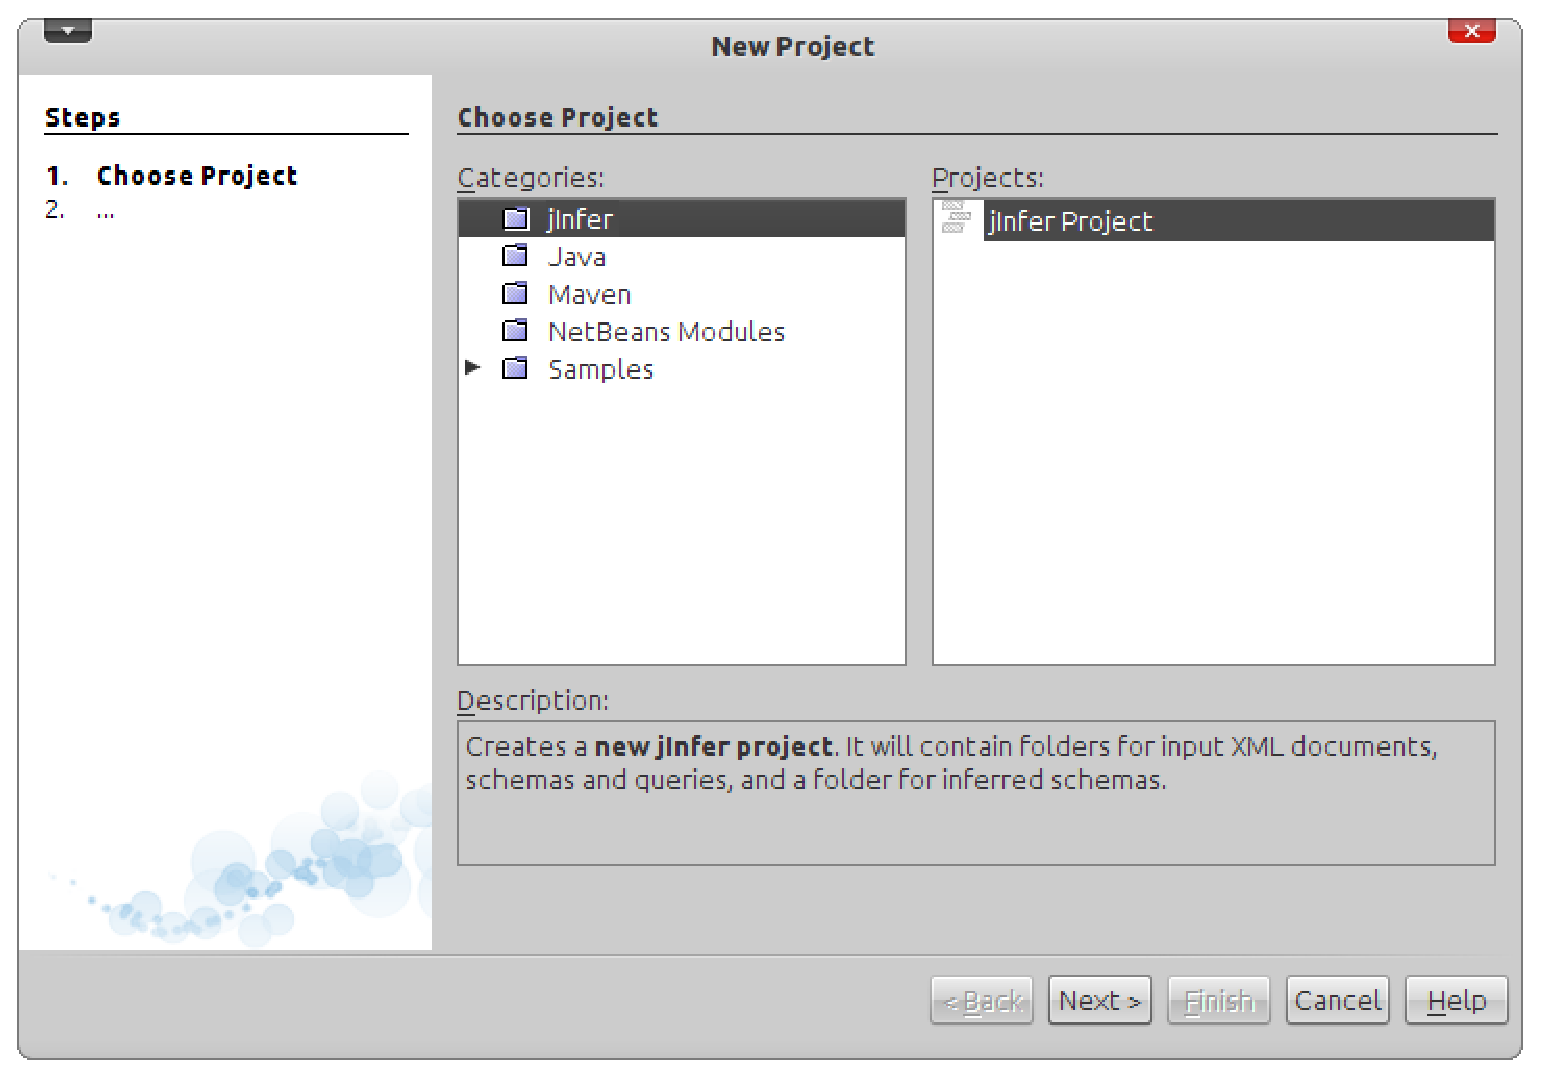
\includegraphics[width=\textwidth]{tutorial_images/new_project}
\end{figure}

Files with XML data, defined functional dependencies and weights assigned to the nodes needs to be added to the newly created project. Files with functional dependencies and weights are xml files with XML Schema shown in Fig. \ref{fdschema} and \ref{weightschema}. These files appears after adding in the \emph{FD} folder of the jInfer project.

\begin{figure}[H]
    \centering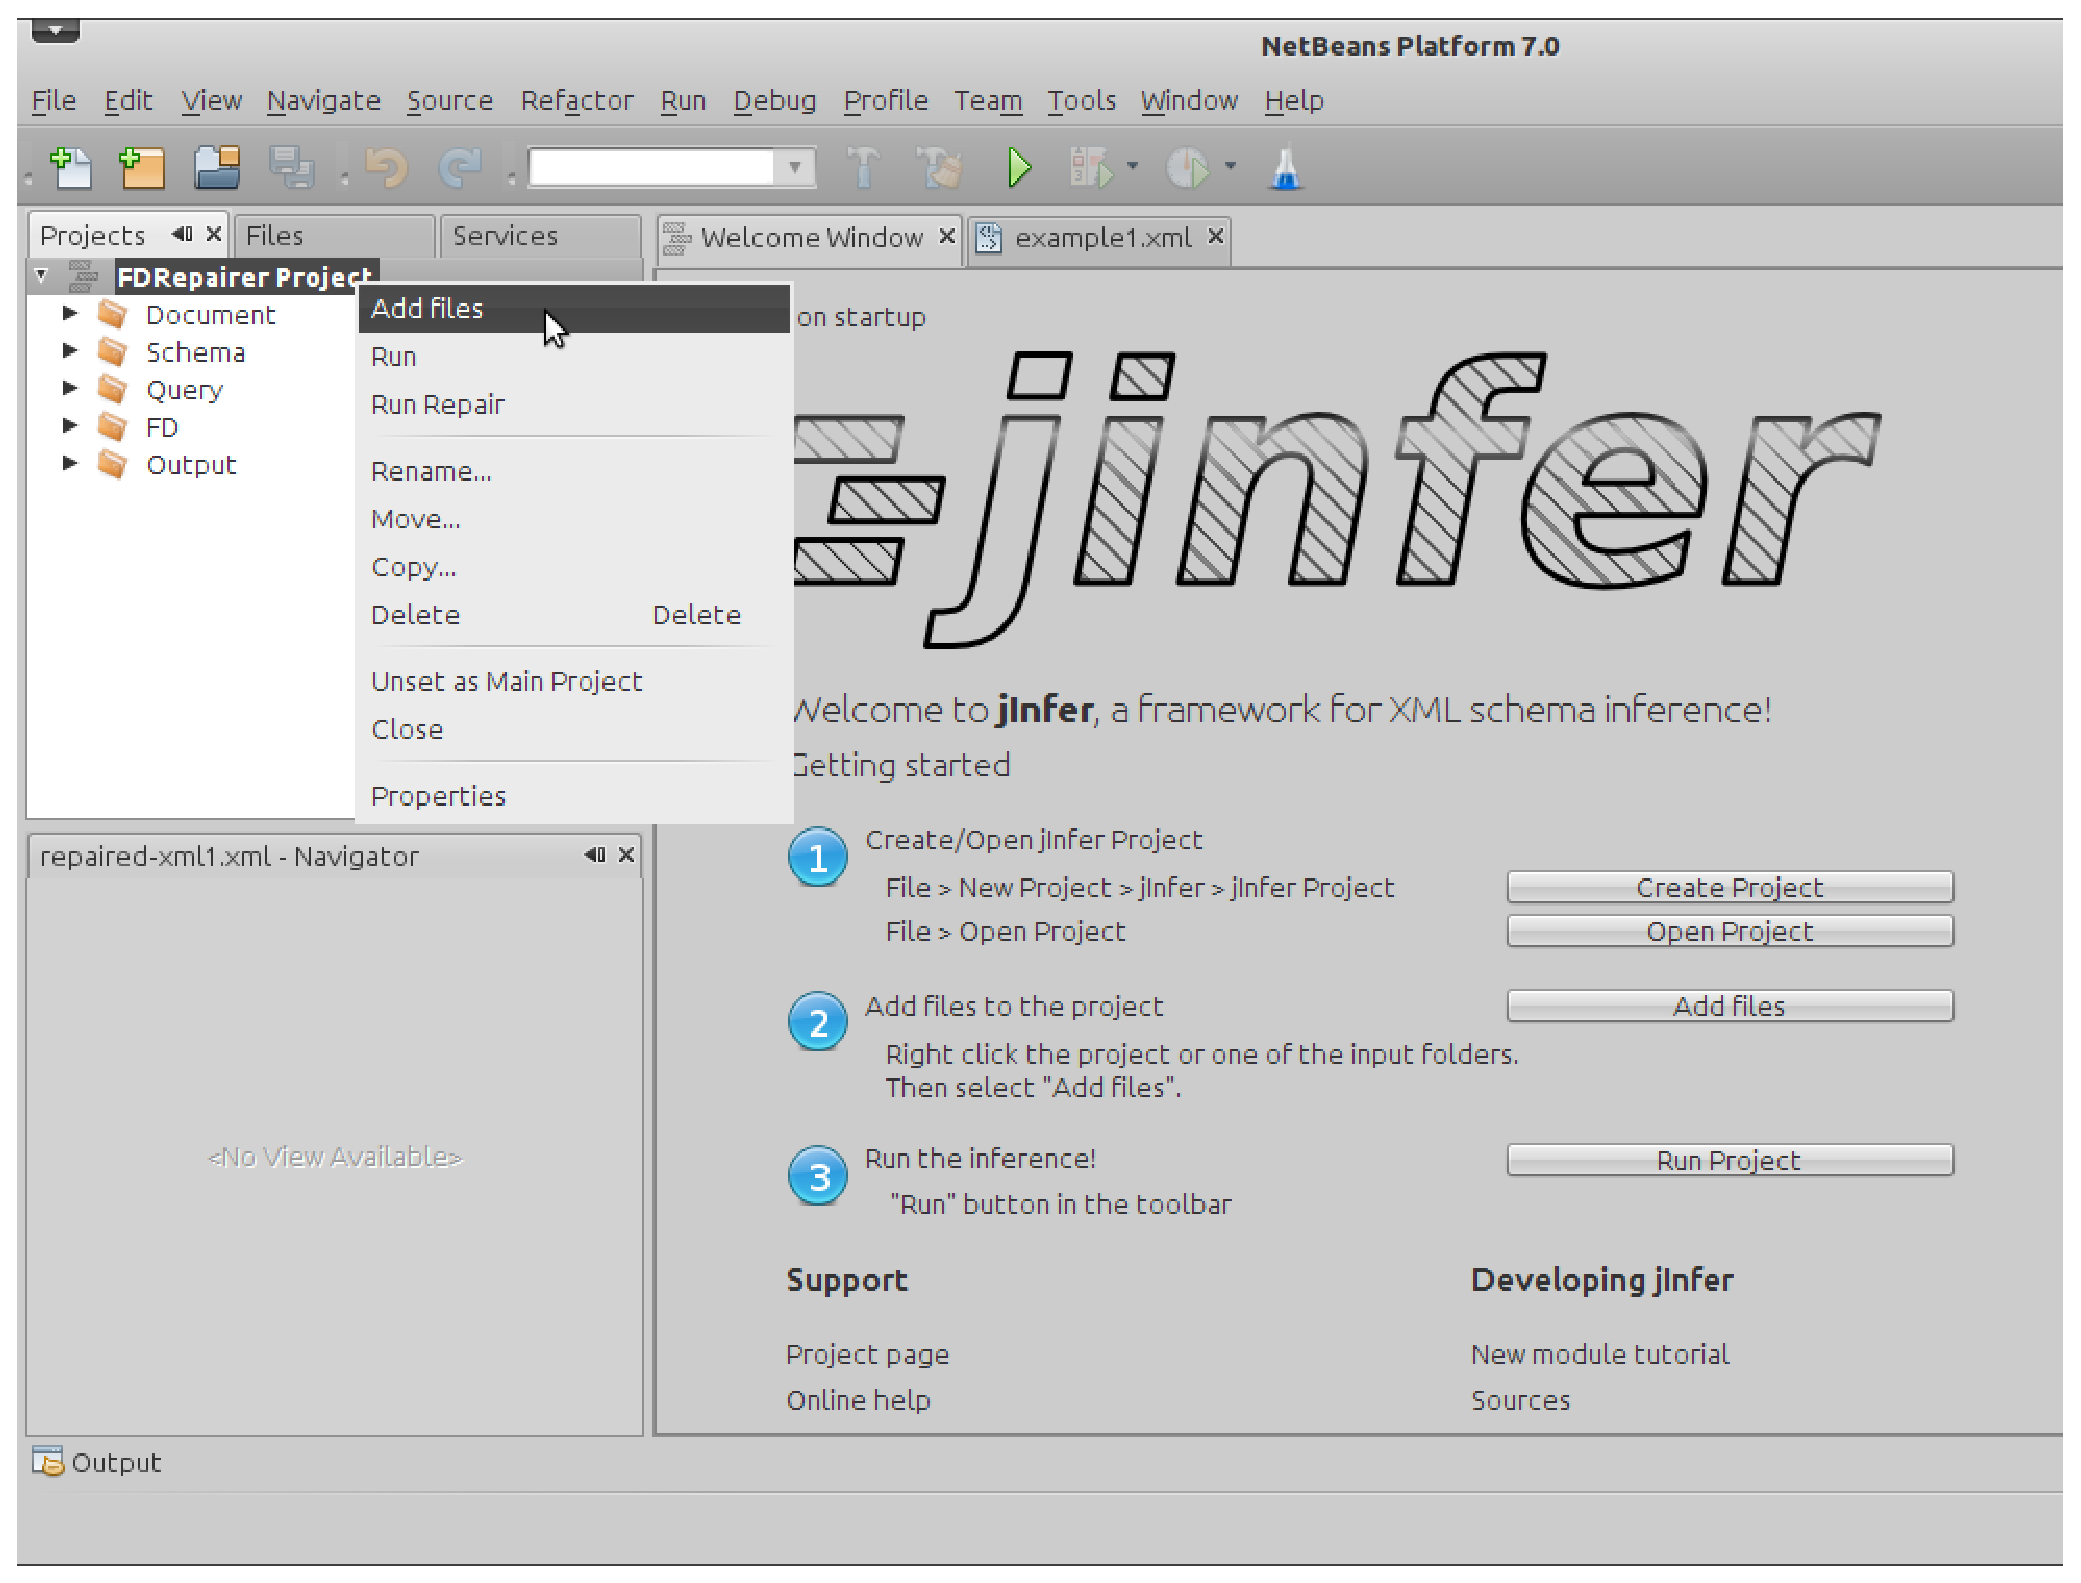
\includegraphics[width=\textwidth]{tutorial_images/add_files}
\end{figure}

The settings of the \texttt{FDRepairer} extension is available in the properties window of the jInfer project accessible through project context menu. In these settings, one could choose between original repairer and repairer proposed in this thesis. For the proposed algorithm is then available to choose between \emph{user interactive} repair picker and \emph{Minimal Repair Picker}. In this place is also possible to set coefficient $k$ and threshold $t$.

\begin{figure}[H]
    \centering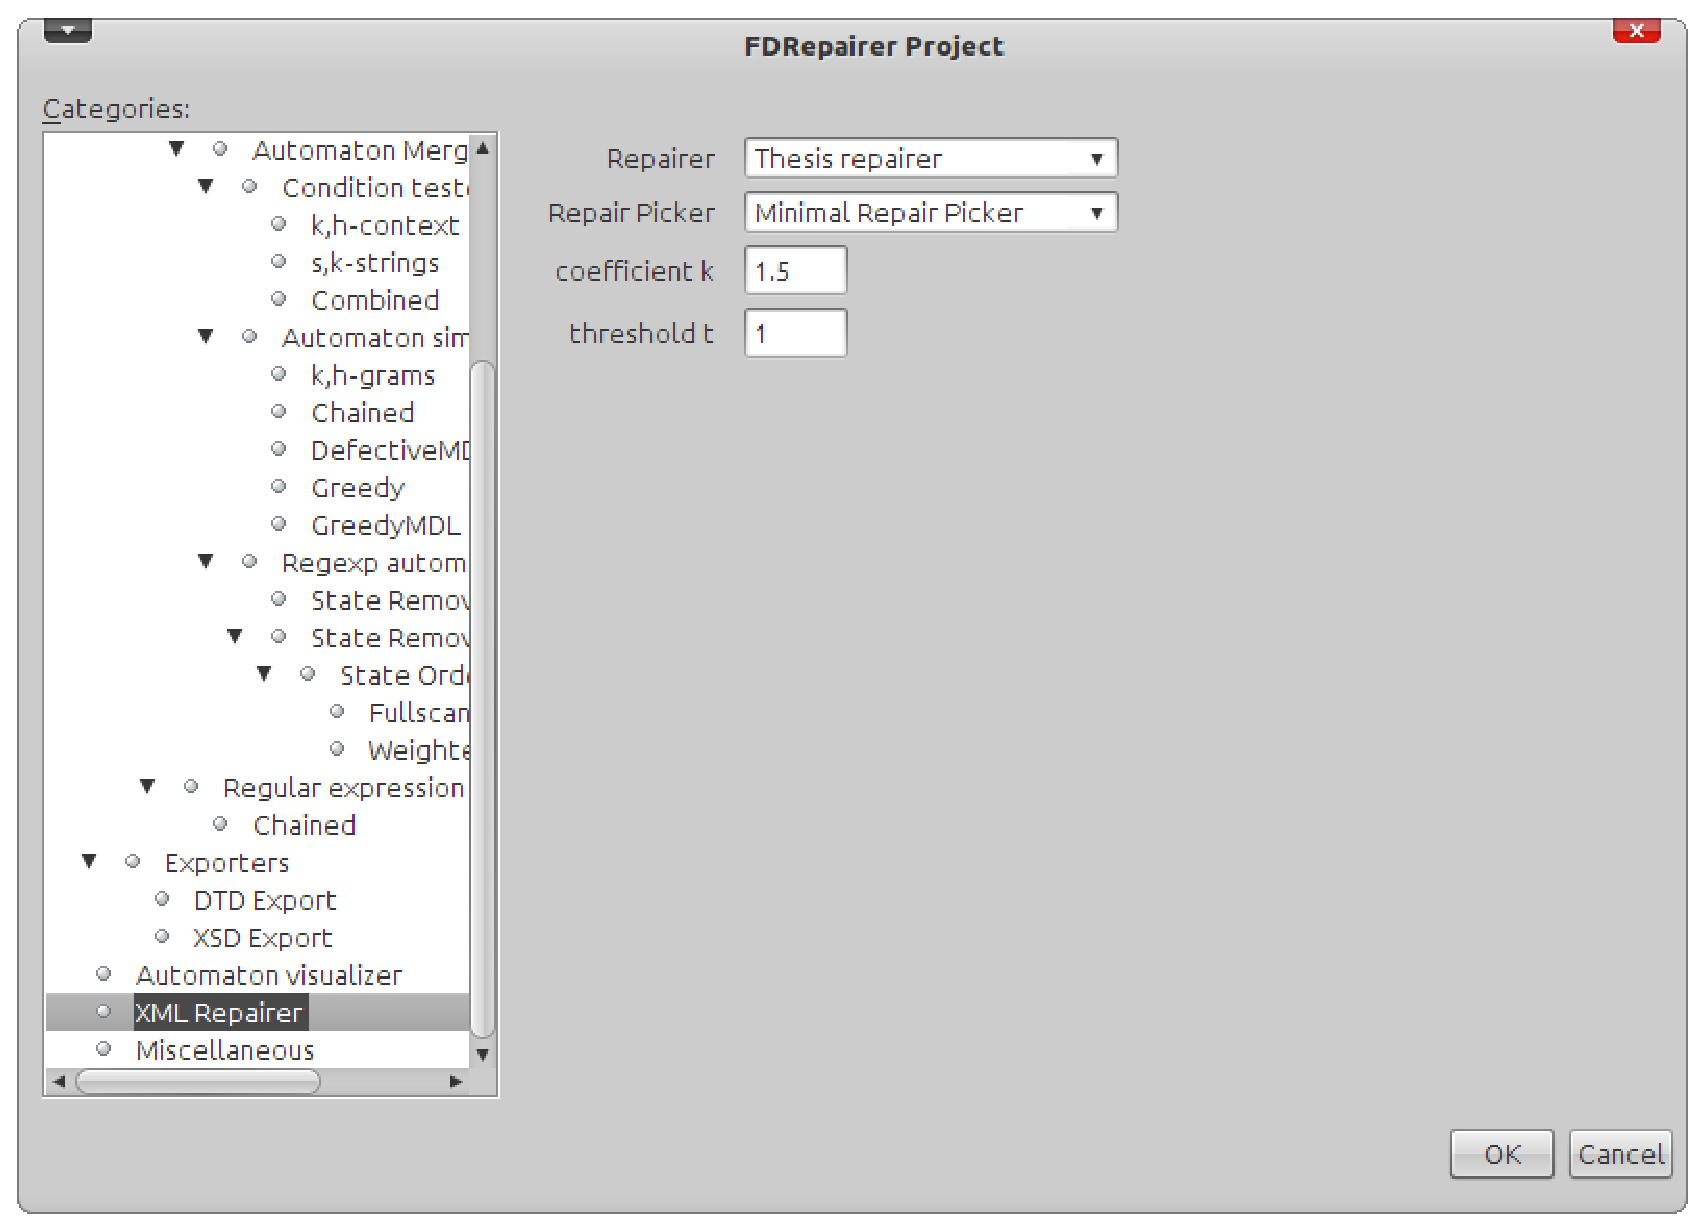
\includegraphics[width=\textwidth]{tutorial_images/project_properties}
\end{figure}

The repair is executed by the \emph{Run Repair} item from the jInfer project context menu:

\begin{figure}[H]
    \centering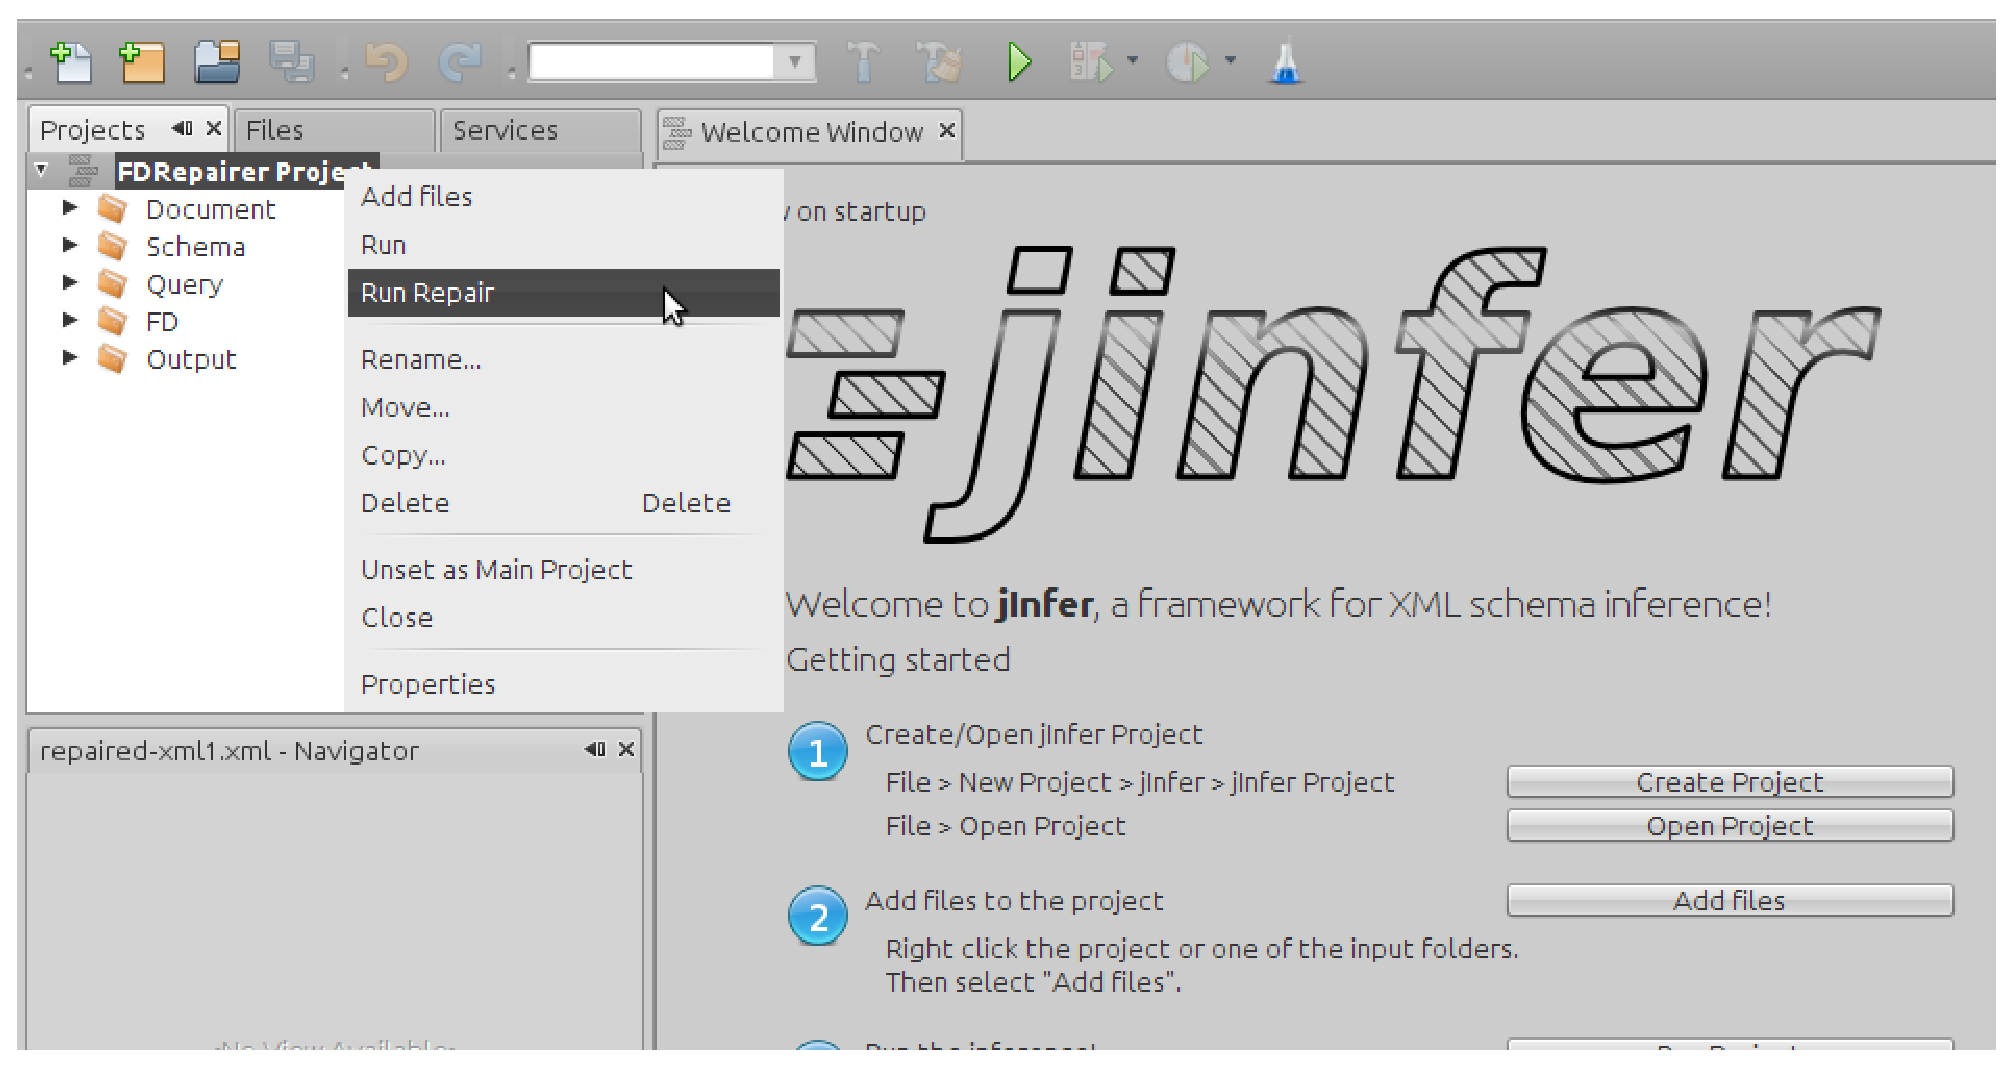
\includegraphics[width=\textwidth]{tutorial_images/run_repair}
\end{figure}

If the \emph{user interactive} repair picker has been selected, \emph{RepairPicker Window} is shown to the user. In this window the user picks repair candidate, which will be applied to the repaired XML.

\begin{figure}[H]
    \centering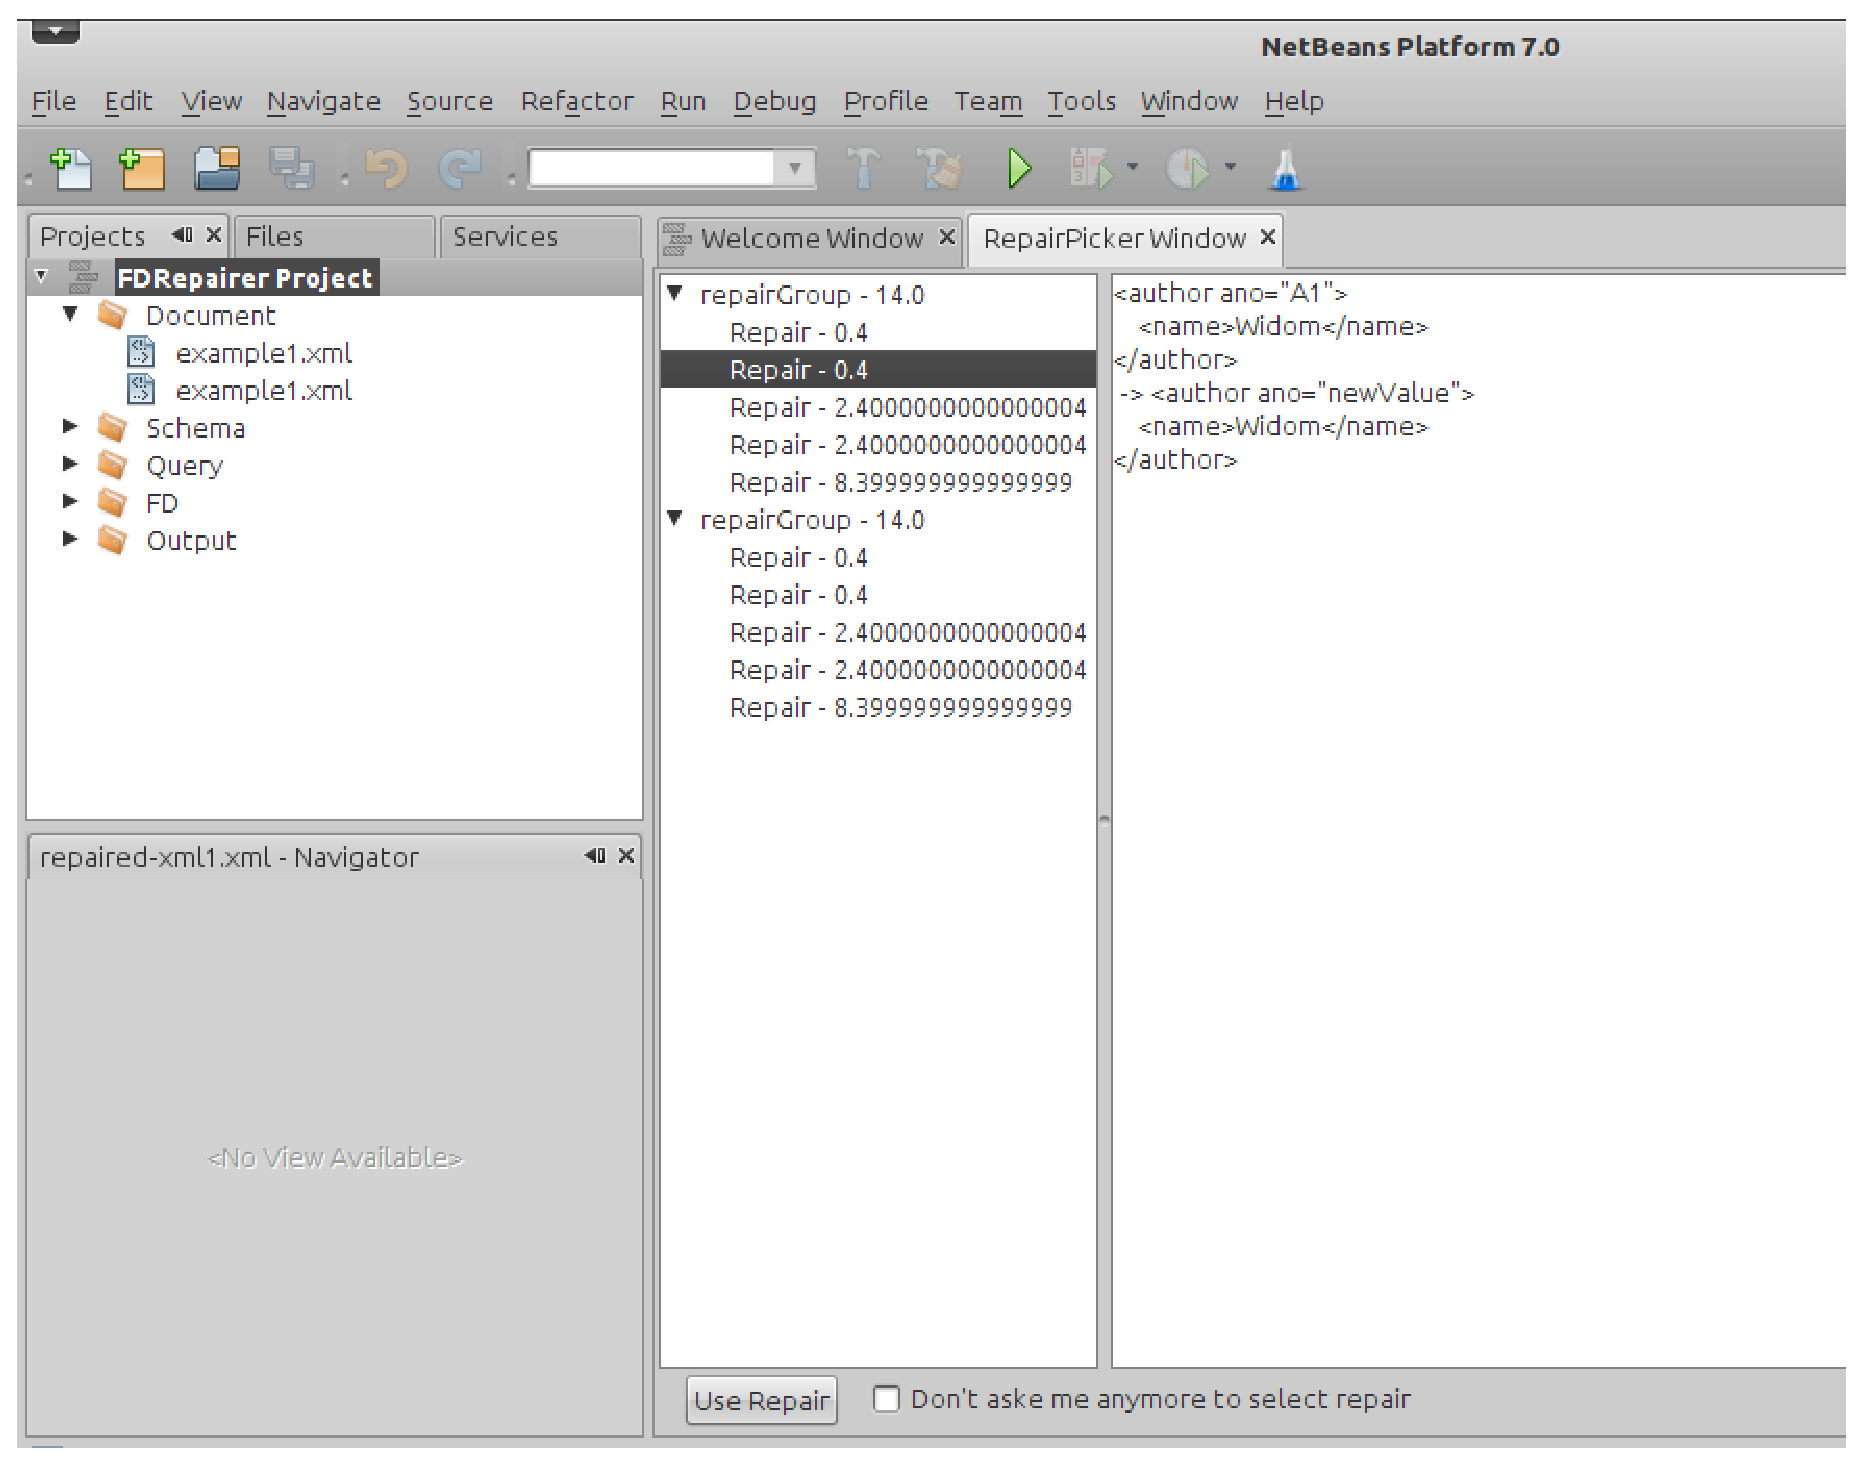
\includegraphics[width=\textwidth]{tutorial_images/user_selection}
\end{figure}

After repairing all the violations, repaired XML document is created in the \emph{Output} subfolder of the jInfer project.


\openright
\end{document}
